% Options for packages loaded elsewhere
\PassOptionsToPackage{unicode}{hyperref}
\PassOptionsToPackage{hyphens}{url}
\PassOptionsToPackage{dvipsnames,svgnames,x11names}{xcolor}
%
\documentclass[
  letterpaper,
  DIV=11,
  numbers=noendperiod]{scrreprt}

\usepackage{amsmath,amssymb}
\usepackage{iftex}
\ifPDFTeX
  \usepackage[T1]{fontenc}
  \usepackage[utf8]{inputenc}
  \usepackage{textcomp} % provide euro and other symbols
\else % if luatex or xetex
  \usepackage{unicode-math}
  \defaultfontfeatures{Scale=MatchLowercase}
  \defaultfontfeatures[\rmfamily]{Ligatures=TeX,Scale=1}
\fi
\usepackage{lmodern}
\ifPDFTeX\else  
    % xetex/luatex font selection
\fi
% Use upquote if available, for straight quotes in verbatim environments
\IfFileExists{upquote.sty}{\usepackage{upquote}}{}
\IfFileExists{microtype.sty}{% use microtype if available
  \usepackage[]{microtype}
  \UseMicrotypeSet[protrusion]{basicmath} % disable protrusion for tt fonts
}{}
\makeatletter
\@ifundefined{KOMAClassName}{% if non-KOMA class
  \IfFileExists{parskip.sty}{%
    \usepackage{parskip}
  }{% else
    \setlength{\parindent}{0pt}
    \setlength{\parskip}{6pt plus 2pt minus 1pt}}
}{% if KOMA class
  \KOMAoptions{parskip=half}}
\makeatother
\usepackage{xcolor}
\setlength{\emergencystretch}{3em} % prevent overfull lines
\setcounter{secnumdepth}{5}
% Make \paragraph and \subparagraph free-standing
\ifx\paragraph\undefined\else
  \let\oldparagraph\paragraph
  \renewcommand{\paragraph}[1]{\oldparagraph{#1}\mbox{}}
\fi
\ifx\subparagraph\undefined\else
  \let\oldsubparagraph\subparagraph
  \renewcommand{\subparagraph}[1]{\oldsubparagraph{#1}\mbox{}}
\fi


\providecommand{\tightlist}{%
  \setlength{\itemsep}{0pt}\setlength{\parskip}{0pt}}\usepackage{longtable,booktabs,array}
\usepackage{calc} % for calculating minipage widths
% Correct order of tables after \paragraph or \subparagraph
\usepackage{etoolbox}
\makeatletter
\patchcmd\longtable{\par}{\if@noskipsec\mbox{}\fi\par}{}{}
\makeatother
% Allow footnotes in longtable head/foot
\IfFileExists{footnotehyper.sty}{\usepackage{footnotehyper}}{\usepackage{footnote}}
\makesavenoteenv{longtable}
\usepackage{graphicx}
\makeatletter
\def\maxwidth{\ifdim\Gin@nat@width>\linewidth\linewidth\else\Gin@nat@width\fi}
\def\maxheight{\ifdim\Gin@nat@height>\textheight\textheight\else\Gin@nat@height\fi}
\makeatother
% Scale images if necessary, so that they will not overflow the page
% margins by default, and it is still possible to overwrite the defaults
% using explicit options in \includegraphics[width, height, ...]{}
\setkeys{Gin}{width=\maxwidth,height=\maxheight,keepaspectratio}
% Set default figure placement to htbp
\makeatletter
\def\fps@figure{htbp}
\makeatother
\newlength{\cslhangindent}
\setlength{\cslhangindent}{1.5em}
\newlength{\csllabelwidth}
\setlength{\csllabelwidth}{3em}
\newlength{\cslentryspacingunit} % times entry-spacing
\setlength{\cslentryspacingunit}{\parskip}
\newenvironment{CSLReferences}[2] % #1 hanging-ident, #2 entry spacing
 {% don't indent paragraphs
  \setlength{\parindent}{0pt}
  % turn on hanging indent if param 1 is 1
  \ifodd #1
  \let\oldpar\par
  \def\par{\hangindent=\cslhangindent\oldpar}
  \fi
  % set entry spacing
  \setlength{\parskip}{#2\cslentryspacingunit}
 }%
 {}
\usepackage{calc}
\newcommand{\CSLBlock}[1]{#1\hfill\break}
\newcommand{\CSLLeftMargin}[1]{\parbox[t]{\csllabelwidth}{#1}}
\newcommand{\CSLRightInline}[1]{\parbox[t]{\linewidth - \csllabelwidth}{#1}\break}
\newcommand{\CSLIndent}[1]{\hspace{\cslhangindent}#1}

\KOMAoption{captions}{tableheading,figureheading}
\makeatletter
\@ifpackageloaded{tcolorbox}{}{\usepackage[skins,breakable]{tcolorbox}}
\@ifpackageloaded{fontawesome5}{}{\usepackage{fontawesome5}}
\definecolor{quarto-callout-color}{HTML}{909090}
\definecolor{quarto-callout-note-color}{HTML}{0758E5}
\definecolor{quarto-callout-important-color}{HTML}{CC1914}
\definecolor{quarto-callout-warning-color}{HTML}{EB9113}
\definecolor{quarto-callout-tip-color}{HTML}{00A047}
\definecolor{quarto-callout-caution-color}{HTML}{FC5300}
\definecolor{quarto-callout-color-frame}{HTML}{acacac}
\definecolor{quarto-callout-note-color-frame}{HTML}{4582ec}
\definecolor{quarto-callout-important-color-frame}{HTML}{d9534f}
\definecolor{quarto-callout-warning-color-frame}{HTML}{f0ad4e}
\definecolor{quarto-callout-tip-color-frame}{HTML}{02b875}
\definecolor{quarto-callout-caution-color-frame}{HTML}{fd7e14}
\makeatother
\makeatletter
\makeatother
\makeatletter
\@ifpackageloaded{bookmark}{}{\usepackage{bookmark}}
\makeatother
\makeatletter
\@ifpackageloaded{caption}{}{\usepackage{caption}}
\AtBeginDocument{%
\ifdefined\contentsname
  \renewcommand*\contentsname{Table of contents}
\else
  \newcommand\contentsname{Table of contents}
\fi
\ifdefined\listfigurename
  \renewcommand*\listfigurename{List of Figures}
\else
  \newcommand\listfigurename{List of Figures}
\fi
\ifdefined\listtablename
  \renewcommand*\listtablename{List of Tables}
\else
  \newcommand\listtablename{List of Tables}
\fi
\ifdefined\figurename
  \renewcommand*\figurename{Figure}
\else
  \newcommand\figurename{Figure}
\fi
\ifdefined\tablename
  \renewcommand*\tablename{Table}
\else
  \newcommand\tablename{Table}
\fi
}
\@ifpackageloaded{float}{}{\usepackage{float}}
\floatstyle{ruled}
\@ifundefined{c@chapter}{\newfloat{codelisting}{h}{lop}}{\newfloat{codelisting}{h}{lop}[chapter]}
\floatname{codelisting}{Listing}
\newcommand*\listoflistings{\listof{codelisting}{List of Listings}}
\makeatother
\makeatletter
\@ifpackageloaded{caption}{}{\usepackage{caption}}
\@ifpackageloaded{subcaption}{}{\usepackage{subcaption}}
\makeatother
\makeatletter
\@ifpackageloaded{tcolorbox}{}{\usepackage[skins,breakable]{tcolorbox}}
\makeatother
\makeatletter
\@ifundefined{shadecolor}{\definecolor{shadecolor}{rgb}{.97, .97, .97}}
\makeatother
\makeatletter
\makeatother
\makeatletter
\makeatother
\ifLuaTeX
  \usepackage{selnolig}  % disable illegal ligatures
\fi
\IfFileExists{bookmark.sty}{\usepackage{bookmark}}{\usepackage{hyperref}}
\IfFileExists{xurl.sty}{\usepackage{xurl}}{} % add URL line breaks if available
\urlstyle{same} % disable monospaced font for URLs
\hypersetup{
  pdftitle={ASA Methods Manual (version 0.1)},
  colorlinks=true,
  linkcolor={blue},
  filecolor={Maroon},
  citecolor={Blue},
  urlcolor={Blue},
  pdfcreator={LaTeX via pandoc}}

\title{ASA Methods Manual (version 0.1)}
\author{}
\date{2023-09-12}

\begin{document}
\maketitle
\ifdefined\Shaded\renewenvironment{Shaded}{\begin{tcolorbox}[interior hidden, boxrule=0pt, breakable, enhanced, borderline west={3pt}{0pt}{shadecolor}, sharp corners, frame hidden]}{\end{tcolorbox}}\fi

\renewcommand*\contentsname{Table of contents}
{
\hypersetup{linkcolor=}
\setcounter{tocdepth}{2}
\tableofcontents
}
\bookmarksetup{startatroot}

\hypertarget{preface}{%
\chapter*{Preface}\label{preface}}
\addcontentsline{toc}{chapter}{Preface}

\markboth{Preface}{Preface}

This manual represents the methods used to develop the American Society
of Anesthesiologists (ASA) practice parameters. It describes processes,
procedures, and relevant policies overseen by the Committee on Practice
Parameters (CPP).

As the methods and approaches evolve, modification are incorporated.
Those representing ASA policy or falling under CPP's authority are
included only after administrative approval (eg, matters related to
conflict of interest or the choice of strength of evidence framework).
Other changes, for example evidence synthesis methods, are the purview
of methodologists. They are updated as appropriate or when
clarifications are necessary. A history of substantive modifications are
listed at the end of each chapter (in the online version only).

Comments, suggestions for additions, or corrections can be sent to
\href{mailto:m.grant@asahq.org}{Mark Grant}.

\bookmarksetup{startatroot}

\hypertarget{introduction}{%
\chapter{Introduction}\label{introduction}}

\hypertarget{background}{%
\section{Background}\label{background}}

Practice parameters are ``strategies for patient management developed by
the profession to assist physicians in clinical decision making''
(Health Subcommittee Hearing, 1990). The methods described here apply to
the development of ASA Practice Guidelines and Practice Advisories. They
are similar in approach and methodologies but differ in that the
evidence included in Advisories is limited in overall quantity, quality,
and consistency. Classifying a guidance document as a Practice Advisory
is accordingly based on the supporting systematic review. Differences
notwithstanding, both types of guidance adhere to standards for
trustworthy clinical practice guidelines (Graham, 2011).

The first ASA Practice Guidelines, published in 1993, included
management of the difficult airway (Caplan et al., 1993) and pulmonary
artery catheterization (Roizen et al., 1993). Initial guideline
development followed an approach outlined in the Manual for Clinical
Practice Guideline Development (Woolf, 1991) commissioned by the Agency
for Health Care Policy and Research\footnote{Predecessor to the Agency
  for Healthcare Research and Quality (AHRQ).}. The approach was state
of the art for guideline development at the time detailing 59 steps
accompanied by worksheets, table formats, meeting schedules, and goals.
While many of those steps became standard practice in ASA guideline
development, others were omitted or modified. Over time, some changes to
the guideline development process occurred slowly, while others were
more frequent, including the strength of evidence ratings (1999, 6
categories;\footnote{Supportive, suggestive, equivocal, insufficient,
  inconclusive, silent.} 2009, 5 categories;\footnote{A: supportive
  literature, B: suggestive literature, C: equivocal literature, D:
  insufficient evidence from literature, Inadequate.}⁠ 2010, 4
categories;\footnote{A: supportive literature, B: suggestive literature,
  C: equivocal literature, D: insufficient evidence from literature.}
2013, 3 categories\footnote{Category A, Category B, Insufficient
  Evidence.}). ⁠

Following the release of Clinical Practice Guidelines we can Trust
(Graham, 2011) from the National Academy of Medicine and Finding What
Works in Health Care: Standards for Systematic Review (Eden, 2011),
scrutiny of guideline development increased. In that context, the
approach and methods outlined here reflect the evolution of the ASA
practice parameter enterprise and their adherence to current standards.

\hypertarget{overview}{%
\section{Overview}\label{overview}}

Figure~\ref{fig-overview} broadly outlines the structure and main steps
followed in developing recommendation for each question and detailed in
chapters 3 through \textbf{\#} of this manual.

\begin{figure}

\caption{\label{fig-overview}The ASA process of developing
recommendations.}

{\centering 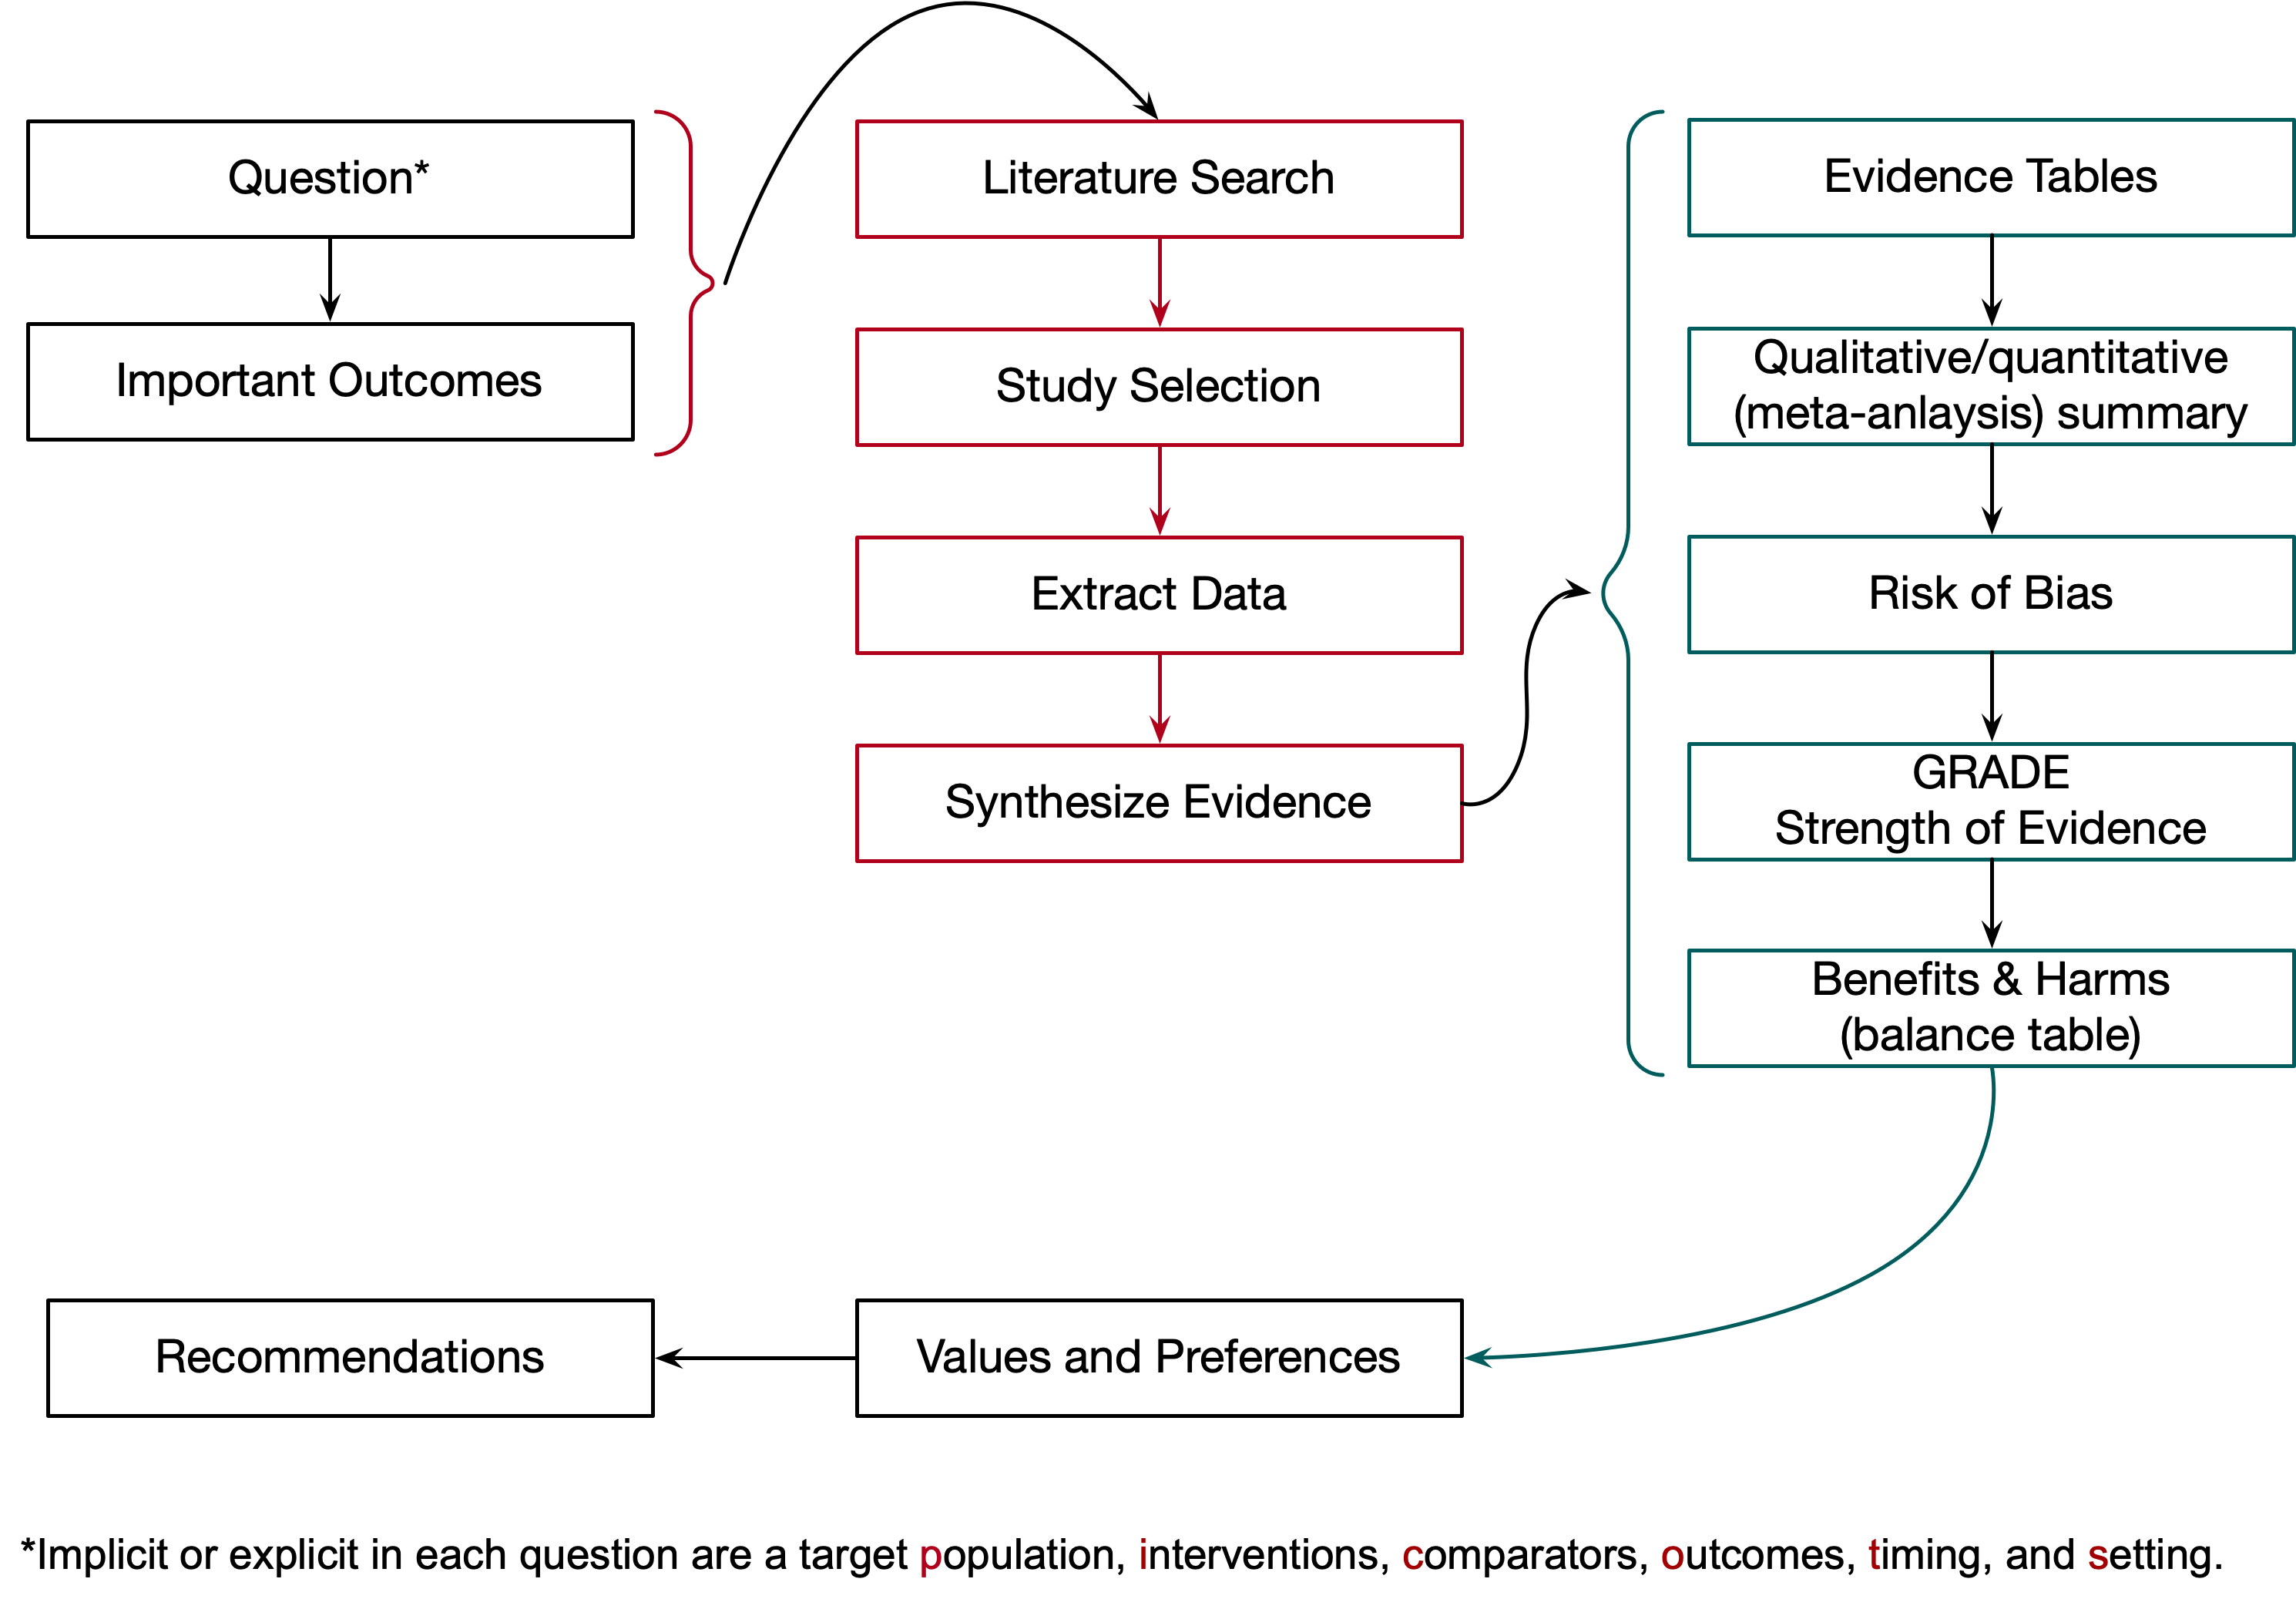
\includegraphics[width=6.25in,height=\textheight]{assets/overview.png}

}

\end{figure}

\bookmarksetup{startatroot}

\hypertarget{organization}{%
\chapter{Organization}\label{organization}}

\hypertarget{committee-on-practice-parameters}{%
\section{Committee on Practice
Parameters}\label{committee-on-practice-parameters}}

The Committee on Practice Parameters (CPP) oversees the development of
practice parameters, including topic prioritization, reviewing and
approving drafts, developing relevant policies (eg, conflict of
interest), and evaluating guidelines from other organizations for
endorsement\footnote{The document generally satisfies ASA's guideline
  development requirements, and there is general agreement with all
  recommendations in the document.} or affirmation of value\footnote{Guideline
  or practice parameter has merit and value but does not generally
  satisfy ASA's guideline development requirements, or there is no
  general agreement with all recommendations in the document.}. CPP
members are self-appointed and include six active ASA members
representing geographically diverse areas, adjunct member(s), and ex
officio members from four quality-focused ASA committees. The chair,
self-appointed with the ASA president's approval, is responsible for
directing and coordinating all committee activities.

\hypertarget{task-forces}{%
\section{Task Forces}\label{task-forces}}

Following a decision to develop a new practice parameter or revise an
existing one, the CPP chair forms a task force. A chair (and optional
co-chair) leads the task force that includes clinicians, patient
representative(s), a librarian/information specialist, methodologists,
and the CPP chair. The clinician members are selected based on
subject-matter expertise, guideline development and review methodology
experience, potential conflicts of interest, and practice diversity. To
minimize potential bias across the task force, membership selection
seeks diversity in sex, gender, race, ethnicity, practice environment,
area of expertise, and geographic region. The task force chair,
co-chairs, and CPP chair oversee practice parameter scope, adherence to
timelines and ASA methodology.

\hypertarget{conflict-of-interest}{%
\section{Conflict of Interest}\label{conflict-of-interest}}

Task force members are required to disclose all personal and immediate
household member\footnote{Partner with whom participant has lived for
  ≥ 1 year in the same home. Dependent or any other related person (by
  blood or marriage) with whom participant has lived for ≥1 year in the
  same home.} relationships with industry and other entities that might
pose a potential conflict of interest. Disclosures cover the 3 years
preceding the first task force meeting and are updated annually through
the year following practice parameter publication. Task force members
are asked to avoid as much as possible changes in potential conflicts of
interest from the time of appointment to the publication. They must
verbally disclose any relevant relationships at the beginning of all
conference calls and meetings. Employees of industry, part- or
full-time, are prohibited from task force membership.

A task force member has a relevant relationship which is considered a
conflict of interest when:

\begin{enumerate}
\def\labelenumi{\arabic{enumi}.}
\item
  The relationship or interest relates to the same or similar subject
  matter, intellectual property, asset, topic, or issue addressed in the
  practice parameter.
\item
  The company/entity with whom the relationship exists makes a drug,
  drug class, or device addressed by the task force makes a drug or
  device that competes for use with a product addressed in the practice
  parameter.
\item
  The person or household member has a reasonable possibility of
  financial, professional, or other personal gains as a result of the
  issues or content addressed by the task force --- and is judged to
  create a risk that a relationship will unduly influence a person's
  judgment.
\end{enumerate}

Chairs and co-chairs, and at least half of the entire task force (chair,
co-chair, other members) must be free of potential conflicts of
interest. Task force members without conflicts of interest participate
in discussions, drafting, and voting on recommendations. Members with
potential conflicts participate in discussions and drafting of
documents, but are recused from voting on recommendations related to
those conflicts.

The disclosure policy can be viewed
\href{assets/CPP_Disclosure_Policy_2022-09-23.pdf}{here}.

\hypertarget{practice-parameter-nomination-and-prioritization}{%
\section{Practice Parameter Nomination and
Prioritization}\label{practice-parameter-nomination-and-prioritization}}

The process of deciding practice parameters to update or develop is
outlined in Figure~\ref{fig-prioritization}. Existing practice
parameters are prioritized annually for updating by ASA leadership, the
Anesthesia Patient Safety Foundation (APSF), committee chairs, and CPP
members. Topic nominations are solicited from ASA leadership, committee
chairs, and APSF in a standardized format. Nominations for new practice
parameters are also accepted from others at any time (sent to the CPP
chair or submitted to \href{mailto:Guidelines@asahq.org}{ASA Standards
and Guidelines}; see
\href{assets/Nomination_Template_2023-07-24.pdf}{template} for suggested
content).

Applying evaluation criteria (separate criteria for updating practice
parameters and new topics) developed by CPP members, the committee next
reviews potential practice parameter updates given the prioritization
survey results and new topic nominations. In a final survey conducted
following the meeting, each CPP member ranks four top choices.

\begin{figure}

\caption{\label{fig-prioritization}Depiction of the prioritization
process.}

{\centering 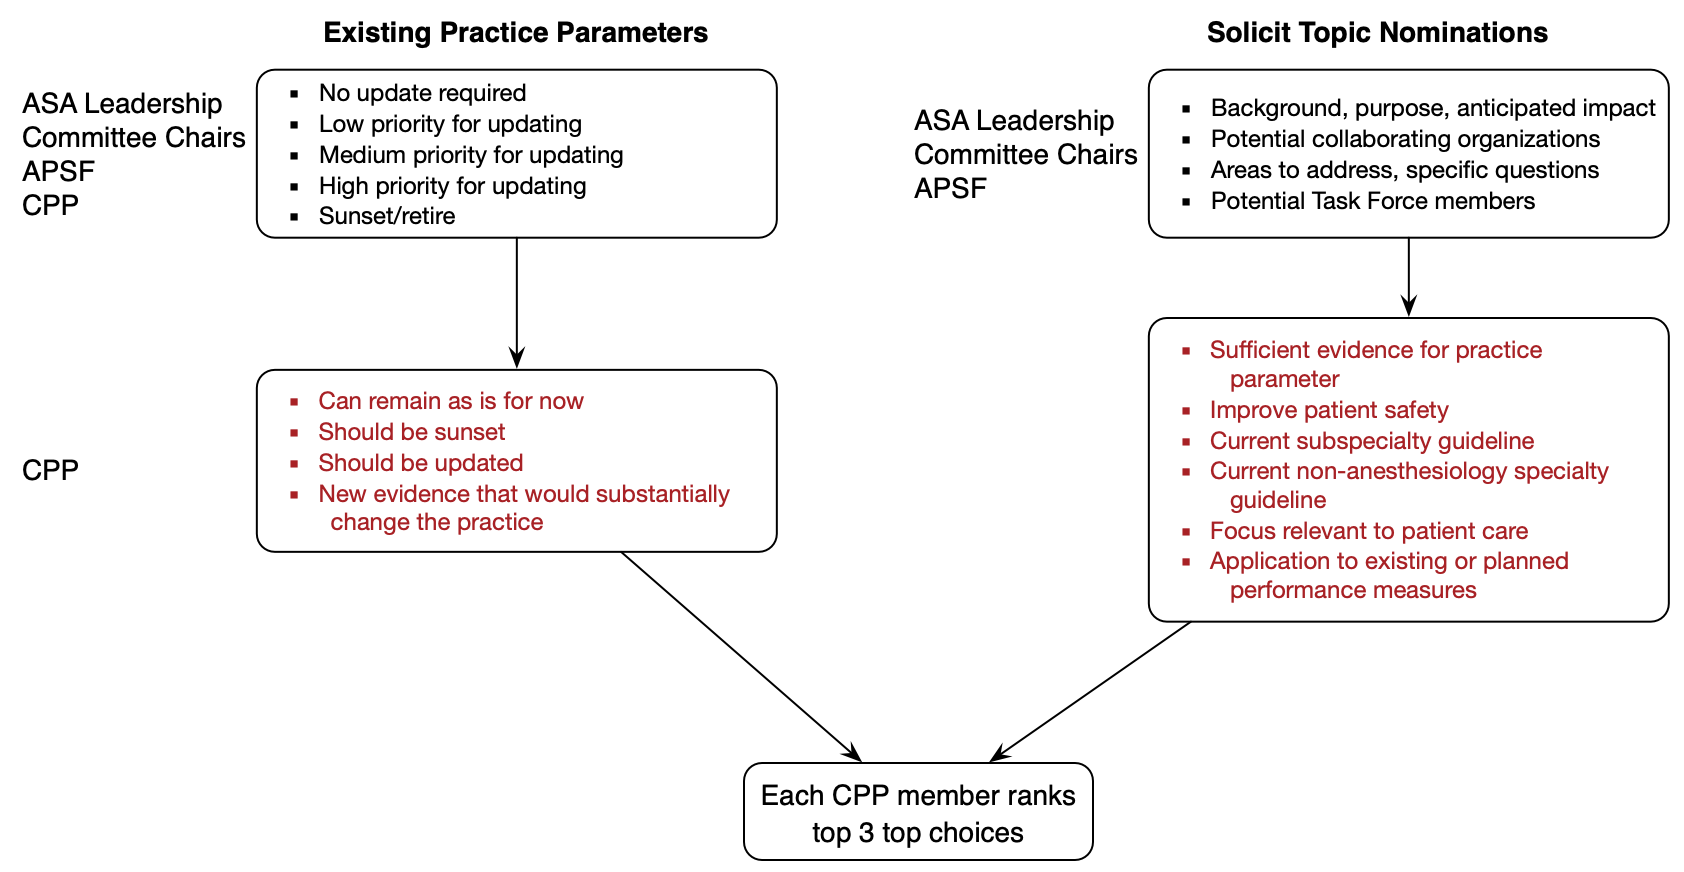
\includegraphics[width=1\textwidth,height=\textheight]{assets/prioritization.png}

}

\end{figure}

\hypertarget{developing-practice-parameters}{%
\section{Developing Practice
Parameters}\label{developing-practice-parameters}}

Figure~\ref{fig-process} outlines the practice parameter development
process. An introductory meeting serves to orient the task force chairs
and co-chairs to the process, timeline, and the roles of methodologists.
Subsequent task force meetings are then devoted to defining the PICOs
(populations, interventions, comparators, and outcomes) and key
questions questions. A protocol is then drafted by the methodologists
and reviewed by the task force 2 to 4 weeks later. The systematic review
and evidence synthesis is then conducted, during which time the task
force is convened as needed for input and decisions concerning any
issues that arise including modifications to the protocol. The
methodologists complete the evidence synthesis to inform
recommendations. Finally, the practice parameter is drafted, submitted
to Anesthesiology for review, public comment is solicited, followed by
submission to the ASA Board of Directors for approval and finally the
House of Delegates.

\begin{figure}

\caption{\label{fig-process}Depiction of the practice parameter
development process.}

{\centering 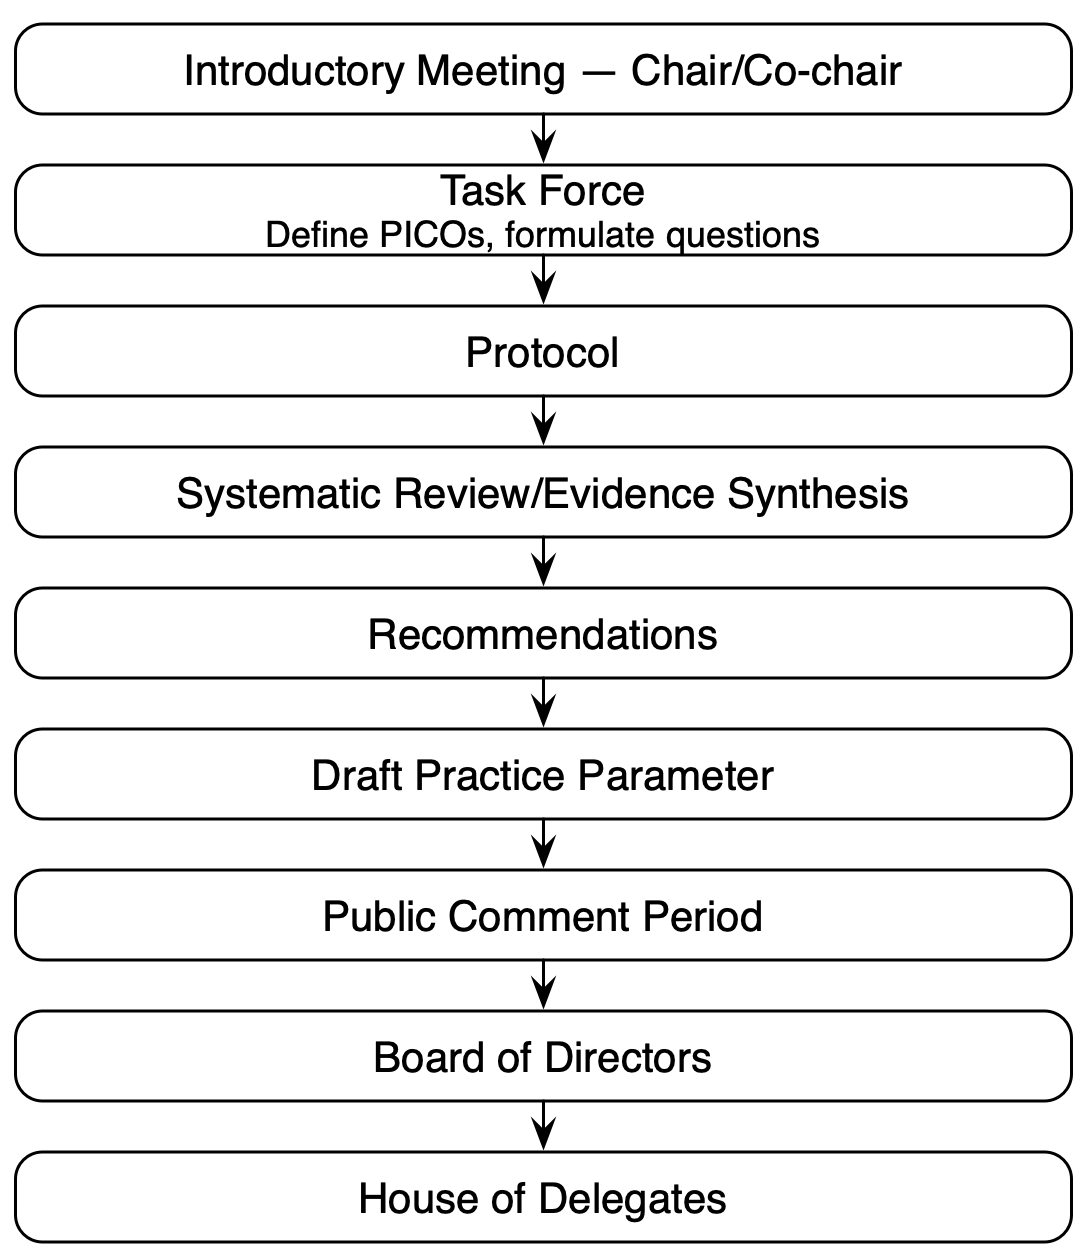
\includegraphics[width=0.4\textwidth,height=\textheight]{assets/process.png}

}

\end{figure}

\bookmarksetup{startatroot}

\hypertarget{systematic-review}{%
\chapter{Systematic Review}\label{systematic-review}}

Trustworthy clinical practice guidelines (Graham, 2011) are supported by
systematic reviews meeting explicit standards (Eden, 2011; PCORI, 2019).
The systematic reviews supporting ASA practice parameters conform to
those standards.

\hypertarget{protocol}{%
\section{Protocol}\label{protocol}}

The protocol, developed collaboratively between the task force and
methodologists, guides systematic review conduct, and provides
documentation for updates. It includes background material, key
questions, PICOTS,\footnote{Populations, interventions, comparators,
  outcomes, timing, and setting.} analytic framework, study inclusion
and exclusion criteria, search strategy, and the anticipated approach to
evidence synthesis. Depending on the anticipated scope, protocols may be
registered on \href{https://www.crd.york.ac.uk/PROSPERO/}{PROSPERO}
(Booth et al., 2012). However, when the systematic review includes
numerous questions and anticipated to require substantial refinement and
modifications, registration is omitted. The protocol is included as a
supplement to the published practice parameter. (An example draft
protocol can be viewed
\href{assets/Protocol_Geriatrics_2022-09-17.pdf}{here}).

\hypertarget{outcome-importance}{%
\section{Outcome Importance}\label{outcome-importance}}

Outcomes vary in importance according to patient values and preferences
(Guyatt et al., 2011). From that perspective, following protocol
completion task force members rate outcome importance for
decision-making. The ratings are reviewed by the entire task force and
revised as necessary to achieve consensus. Outcomes are assigned a level
--- critical, important but not critical, low importance --- and may be
ranked to prioritize conduct of the evidence synthesis.
Figure~\ref{fig-priority} and Figure~\ref{fig-priority_geri} illustrate
the data obtained from ratings and rankings.

\begin{figure}

\caption{\label{fig-priority}Prioritization of outcomes for
neuromuscular monitoring.}

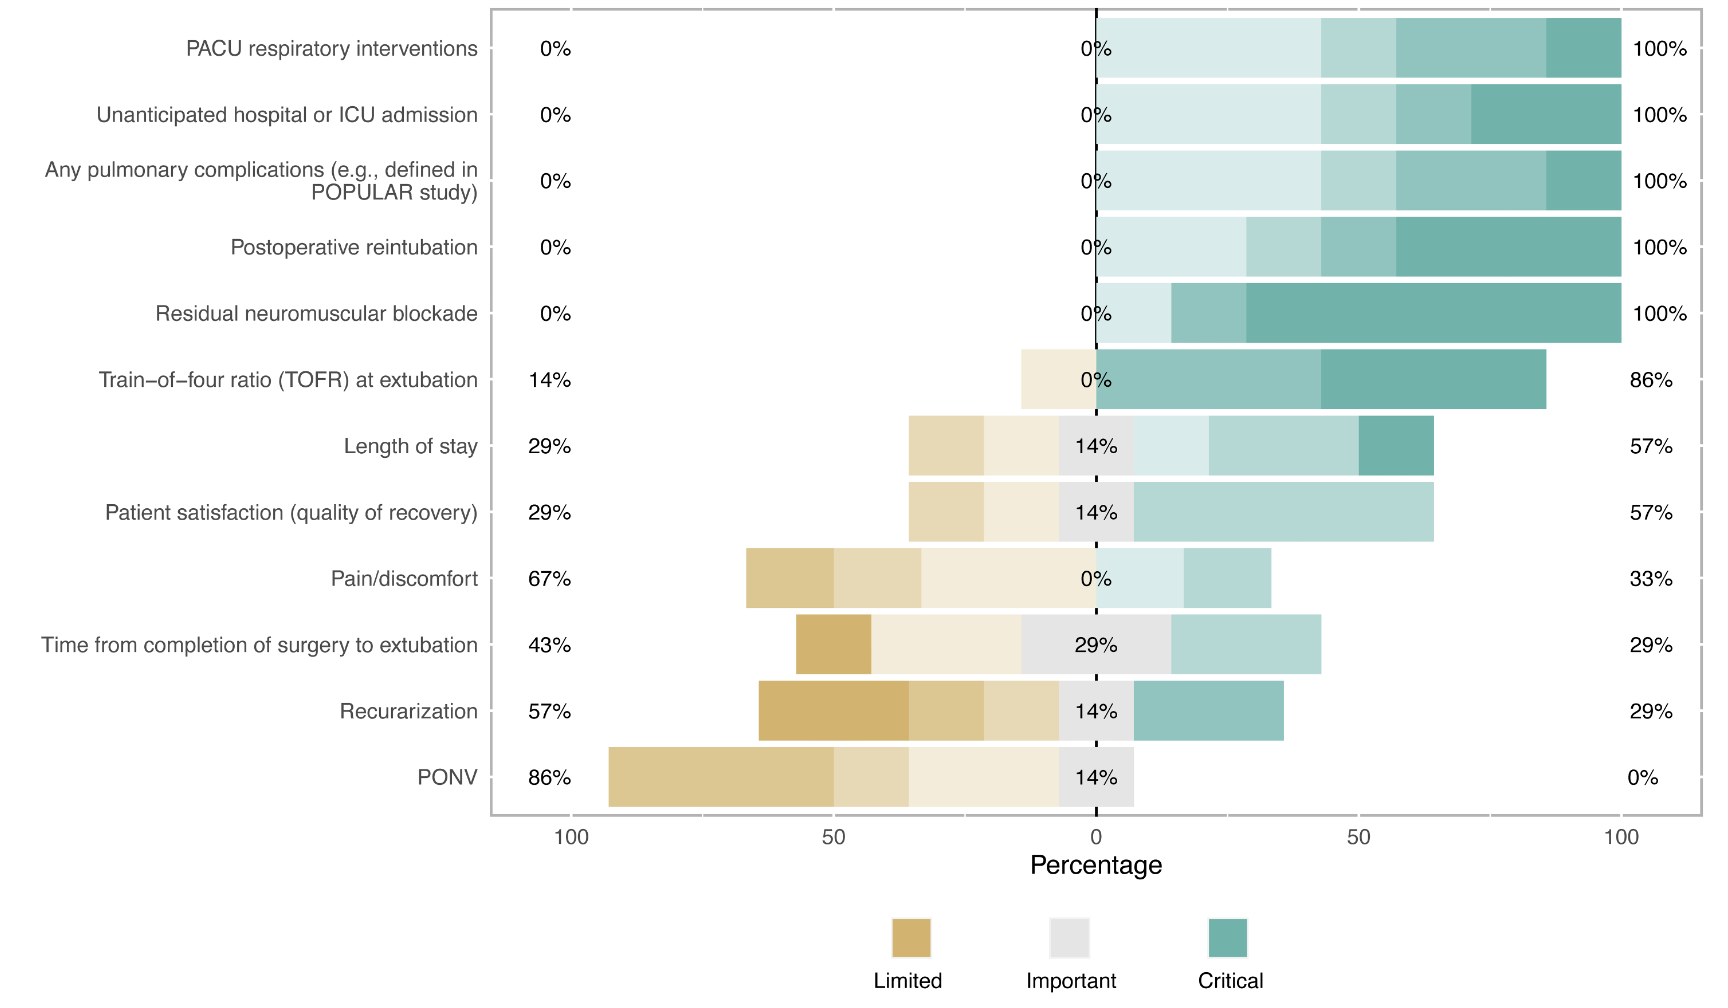
\includegraphics[width=0.9\textwidth,height=\textheight]{assets/priority_nmb.png} \hfill{}

\end{figure}

\begin{figure}

\caption{\label{fig-priority_geri}Example of assessing outcome
importance rankings in a geriatrics guideline. Rankings for the 5 most
important outcomes across 7 key questions (11 respondents with maximum
77 for each outcome rank or any top 5 ranking).}

{\centering 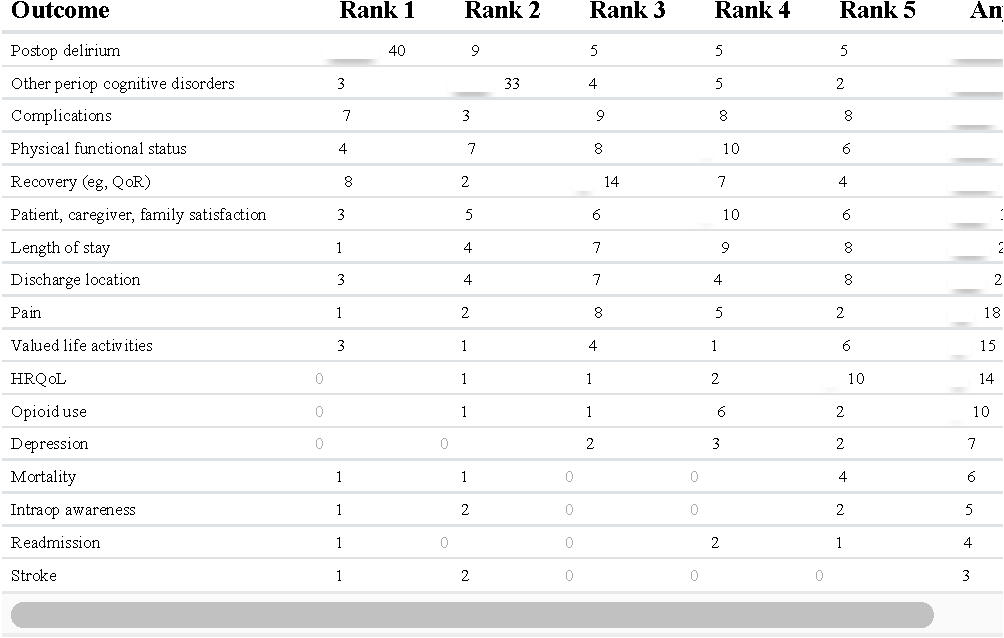
\includegraphics{03_syst_rev_files/figure-pdf/fig-priority_geri-1.pdf}

}

\end{figure}

\emph{Note that rows can be reordered according to ranking by clicking
on column headers.}

\hypertarget{identifying-literature}{%
\section{Identifying Literature}\label{identifying-literature}}

\hypertarget{database-searches}{%
\subsection{Database Searches}\label{database-searches}}

A librarian/information specialist develops search strategies after
reviewing the protocol and participating in task force meetings. The
primary bibliographic databases queried include PubMed, Embase®,
Scopus®, and Cochrane Central Register of Controlled Trials. The task
force also submits relevant references for consideration, including
systematic reviews and guidelines for reference checking. To ensure that
relevant publications have been captured, search result identification
of references submitted by the task force is examined. Grey literature
searches are topic-dependent relying on registries, conference
abstracts, preprint servers, and FDA documents including advisory
meeting transcripts. The search dates are determinied by the task force
and consider sensitivity (Xu et al., 2022), applicability and
generalizability to current practice, and resources required to conduct
the review. Depending on the key question, searches may not be limited
to English language publications (Egger et al., 1997; Jia et al., 2020;
Jüni et al., 2002; Mao et al., 2020).

\hypertarget{citation-searching}{%
\subsection{Citation Searching}\label{citation-searching}}

Backwards searching for studies included in relevant systematic reviews,
meta-analyses, and guidelines are considered eligible for inclusion. The
selection process outlined below (Figure~\ref{fig-checking}) is used to
identify typically 2 to 3 reviews. Studies included in the those reviews
are compiled in a bibliographic database. Those studies not identified
in the primary search are subsequently assessed for eligibility. On a
selective basis, forward citation searching is conducted using seminal
studies to identify citing studies.
\href{https://estech.shinyapps.io/citationchaser/}{Citationchaser}
(Haddaway et al., 2022) and/or
\href{https://paperfetcher-paperfetcher-web-app-paperfetcher-app-0w0vu2.streamlit.app/}{Paperfecter}
(Pallath et al., 2023) are used to facility citation searching.

\begin{figure}

\caption{\label{fig-checking}Approach to backward citation searching.}

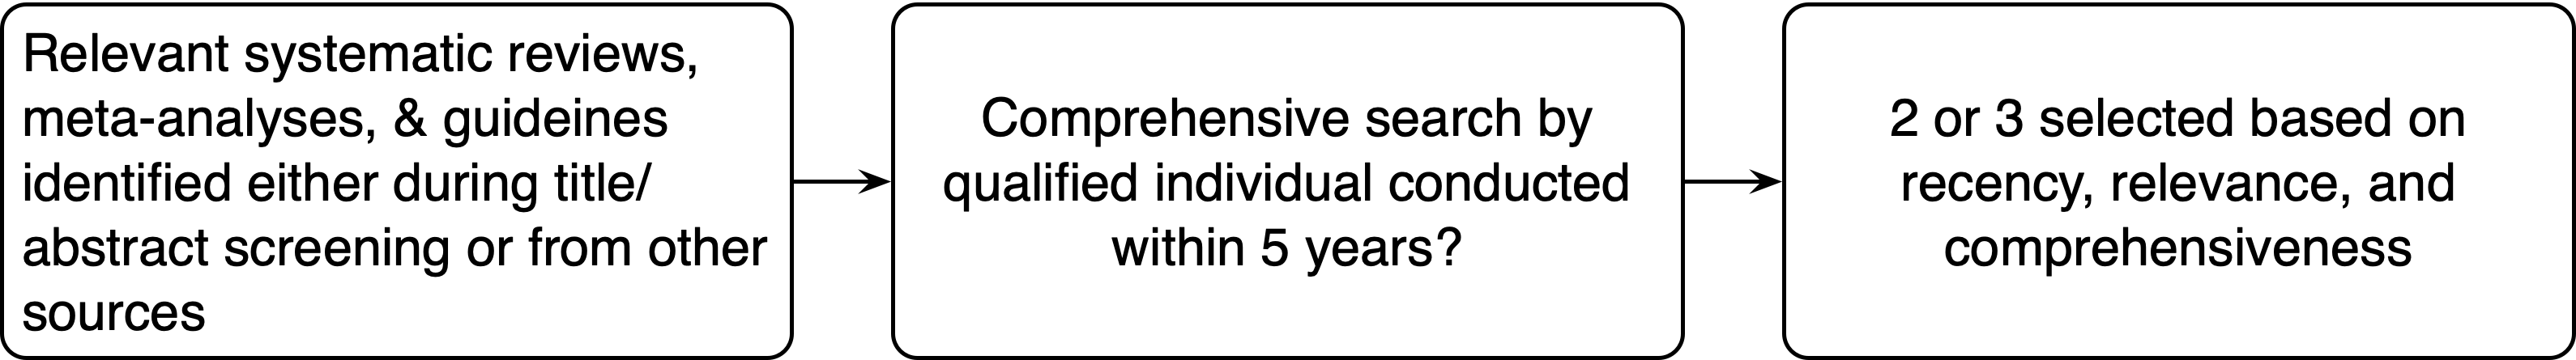
\includegraphics[width=5.20833in,height=\textheight]{assets/referenceChecking.png} \hfill{}

\end{figure}

\hypertarget{task-force}{%
\subsection{Task Force}\label{task-force}}

The task force is given the opportunity to submit potentially relevant
primary studies, guidelines, systematic reviews, and meta-analyses. The
non-primary research are included in the reference checking process and
the remainder considered in the standard selection process.

\hypertarget{retracted-publications}{%
\subsection{Retracted Publications}\label{retracted-publications}}

Identifying retracted publications is critical to assuring the integrity
of the systematic review. Accordingly, searches for retractions of
included studies are conducted using relevant search terms (eg,
\href{https://ambulance.libguides.com/retracted}{see this guide}) and
the
\href{http://retractiondatabase.org/RetractionSearch.aspx?}{Retraction
Watch Database} (can be facilitated using Zotero's
\href{https://www.zotero.org/blog/retracted-item-notifications/}{Retracted
Items} feature).

\hypertarget{deduplication}{%
\subsection{Deduplication}\label{deduplication}}

Deduplication is performed using EndNote™ (used as the primary
bibliographic database) and a dedicated systematic review software
platform (DistillerSR).

\hypertarget{study-selection}{%
\section{Study Selection}\label{study-selection}}

Based on the inclusion-exclusion criteria (study design and PICOTS),
study selection is performed by reviewing titles and abstracts. The
semi-automated predictive tool for title and abstract screening
implemented in DistillerSR is utilized. (Polanin et al., 2019) If the
number of references is exceedingly large (eg, \textgreater{} 10,000 or
15,000), screening may be truncated when inclusion predictions for the
remaining unscreened references are low (eg, less than 2\% to 3\%).
Full-text review of potentially relevant publications is then conducted
with reasons for exclusion at the full-text stage are recorded using a
standard set of justifications.

Study designs considered eligible for specific key questions are
determined by the questions, PICOTS, and evidence availability. For
example, although randomized designs generally offer the most convincing
evidence, if few address a particular question/PICOTS, nonrandomized
designs may be included. Similarly, nonrandomized designs may be
included for evaluation of harms. Case reports and case series,
conference abstracts, letters not considered brief research reports,
non-English publications, and animal studies are generally not
considered eligible.

Two reviewers independently apply inclusion-exclusion criteria at each
stage with discrepancies resolved by consensus including a third
reviewer. Training sets are used to develop agreement concerning the
application of inclusion-exclusion criteria.

\hypertarget{data-extractionmanagement}{%
\section{Data Extraction/Management}\label{data-extractionmanagement}}

Accurate data extraction, quality control, and data management enhance
reproducibility and support valid evidence synthesis. The workflow
standardizes data extraction into a dedicated database with an audit
log, and once entered, minimizes manual data manipulation (eg, cutting
and pasting).

A standard review-specific set of data entry forms, modified for each
systematic review, are used:

\begin{itemize}
\tightlist
\item
  Study characteristics
\item
  Study arm data
\item
  Dichotomous outcomes (as reported)
\item
  Continuous outcomes (as reported)
\item
  Likert or other rating scale outcomes (as reported)
\item
  Risk of bias
\end{itemize}

Data are abstracted by a single reviewer with verification (PCORI, 2019,
pp. SR--1) of data relevant for quantitative synthesis and rating
(GRADEing) the strength of evidence. Figures are digitized as necessary
to obtain results for synthesis. Data are maintained and edited in
DistillerSR, a data dictionary compiled, and then transferred to a local
repository for evidence synthesis or reports created using DistillerSR.
A sample study characteristics form can be seen
\href{assets/studyCharacteristicsGeri.pdf}{here}.

\hypertarget{study-risk-of-bias-assessment}{%
\section{Study Risk of Bias
Assessment}\label{study-risk-of-bias-assessment}}

Risk of bias for individual studies are evaluated using tools relevant
for the study design. The most commonly used tools include:

\begin{itemize}
\tightlist
\item
  Randomized clinical trials ---
  \href{https://sites.google.com/site/riskofbiastool/welcome/rob-2-0-tool/current-version-of-rob-2}{Cochrane
  risk of bias tool 2.0}
\item
  Nonrandomized studies of interventions ---
  \href{https://sites.google.com/site/riskofbiastool/welcome/home}{ROBINS-I}
  (Risk Of Bias In Non-randomized Studies of Interventions)
\item
  Diagnostic studies --
  \href{https://www.bristol.ac.uk/population-health-sciences/projects/quadas/quadas-2/}{QUADAS-2}
  (Quality Assessment of Diagnostic Accuracy Studies)
\end{itemize}

Risk of bias assessments are performed independently by 2 reviews and
discordances in domain and signalling question results reconciled by
consensus including a third reviewer as necessary. Separate risk of bias
assessments are conducted for clinical and patient reported outcomes,
but may not be conducted for each of the typically multiple outcomes
examined.

\bookmarksetup{startatroot}

\hypertarget{evidence-synthesis}{%
\chapter{Evidence Synthesis}\label{evidence-synthesis}}

\hypertarget{introduction-1}{%
\section{Introduction}\label{introduction-1}}

A single study is rarely sufficient to inform a guideline or policy
recommendation\footnote{``It is unusual for a policy question to be
  informed by a single study.''} (Spiegelhalter et al., 2004, p. 267); a
synthesis of evidence obtained from multiple studies is required. The
evidence synthesis may be qualitative or quantitative ranging from
narrative descriptions of study results to pairwise meta-analysis (a
single intervention and comparator) or network meta-analysis (multiple
interventions or comparators). Regardless of the approach, the purpose
of an evidence synthesis is to summarize benefits, harms, and
uncertainty (statistical and non-statistical) to inform decisions and
recommendations.

Figure~\ref{fig-structure} depicts how the evidence synthesis is
structured for each key question and how results support
recommendations. The figure implicitly emphasizes how guideline users
have varied needs with respect to detail. Some are interested only in
recommendations that include no quantitative information. Many
(hopefully most) seek to understand the the summaries detail in the
balance tables. Accordingly, these elements are included in the body of
the published guideline. Others may want to understand details including
GRADE domains, meta-analyses, and how specifics of the synthesis
supports recommendations --- provided as supplementary materials (eg,
see \href{https://mdgrant.github.io/geriatrics_synth/}{example}).
Finally, a rare individual may wish to explore analysis or reproduce
them --- data and code are made available for that purpose.

It should be noted that explanatory text in the guideline is by
necessity more limited than a singular publication devoted to each key
question. However, the degree of detail provided should be sufficient to
allow a transparent view to the most discerning or critical reader.

\begin{figure}

\caption{\label{fig-structure}Schematic of the evidence synthesis in
relation to developing recommendations.}

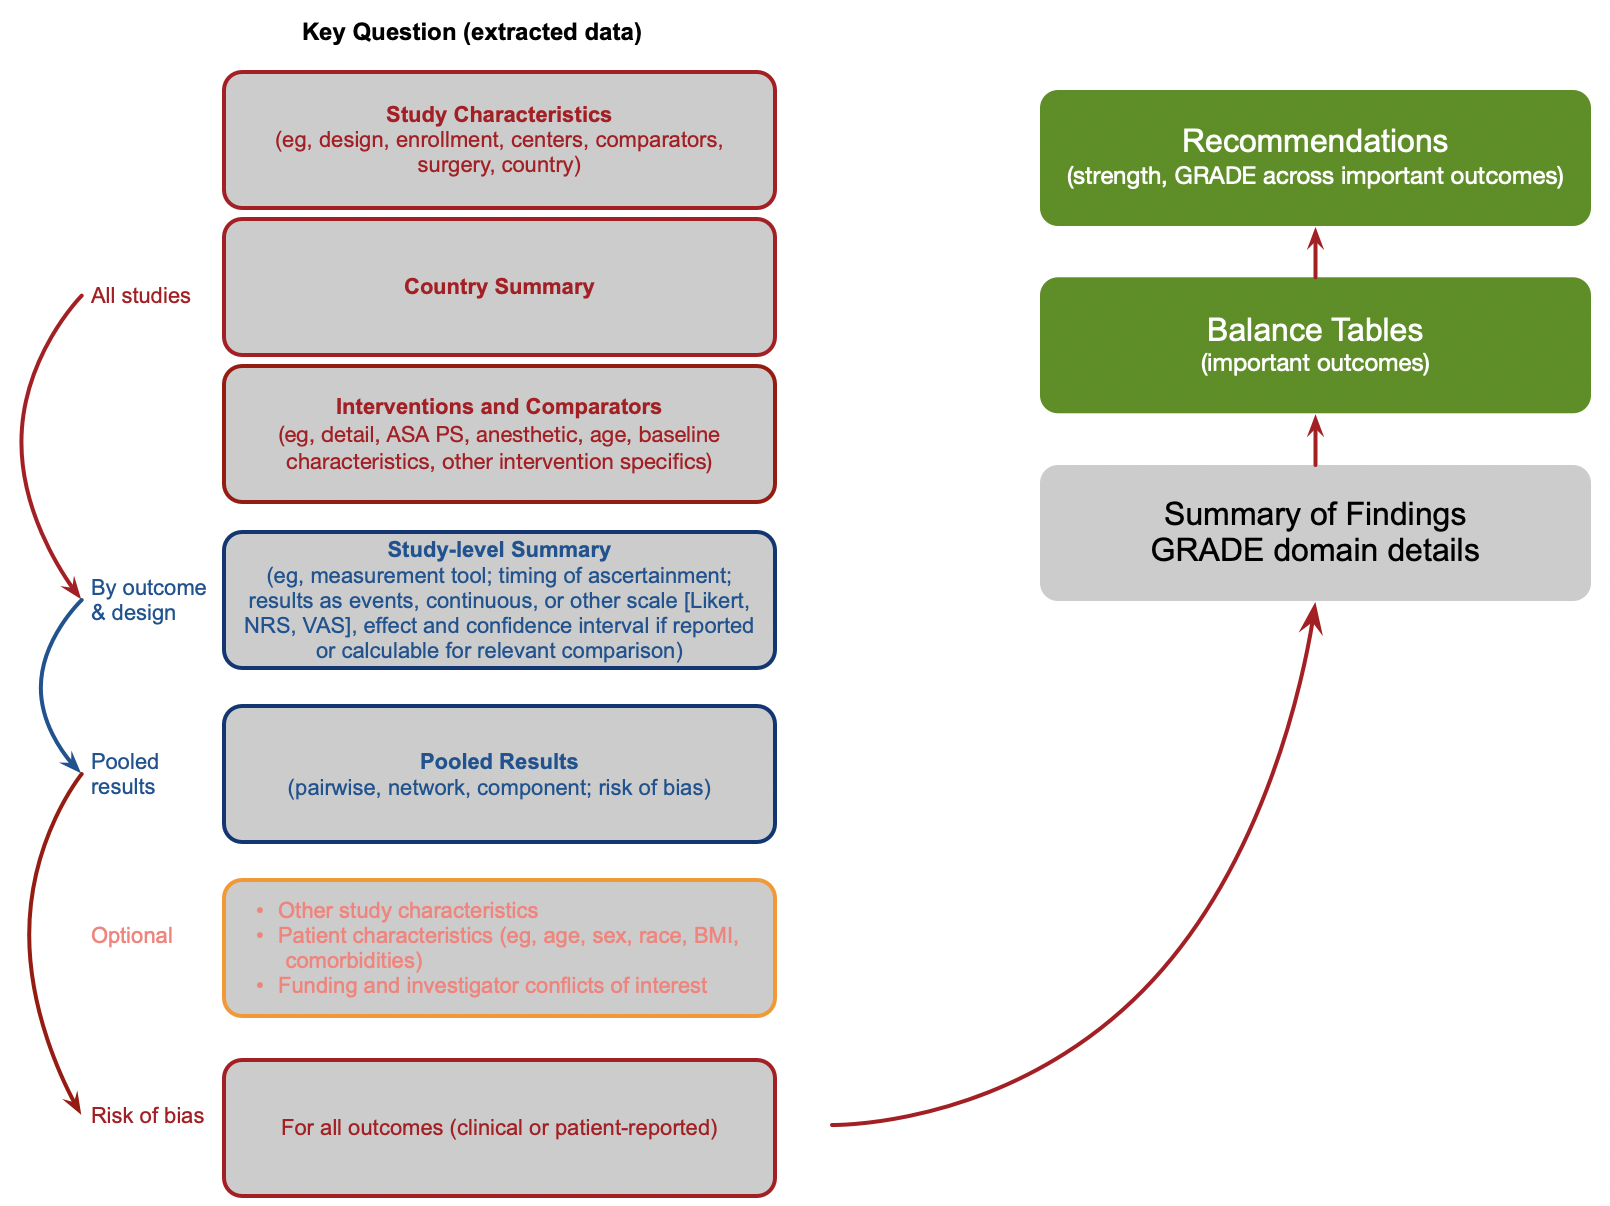
\includegraphics[width=0.75\textwidth,height=\textheight]{assets/structure.png} \hfill{}

\end{figure}

Boxes in gray are included as supplements to the guideline; those in
green are part of the publication.

\hypertarget{decision-making-frameworks}{%
\section{Decision-Making Frameworks}\label{decision-making-frameworks}}

The decision-making required to develop recommendations requires a
framework or model --- a calculus of benefits and harms, how they are
valued, and their respective uncertainties. The explicitness of the
decision calculus varies (Meltzer et al., 2011). For example, a model
can be conceptual existing only in the mind of a decision maker with
little or nothing quantitative. On the other extreme, the model can
decision-analytic with explicit quantitative inputs and outputs. Like
most guideline enterprises, the ASA adopts an approach with qualitative
and quantitative elements between the extremes.

As outlined in Figure~\ref{fig-grade}, after formulating key questions
and important outcomes specified, relevant studies are identified, data
extracted, and risk of bias appraised. Next, using a quantitative or
qualitative synthesis, the strength (certainty/GRADE) of evidence for
each outcome is rated. Outcomes are then weighted according to patient
values and preferences, considered as a whole, and recommendations
formulated.

\begin{figure}

\caption{\label{fig-grade}Model and approach to evidence synthesis for
making recommendations.}

{\centering 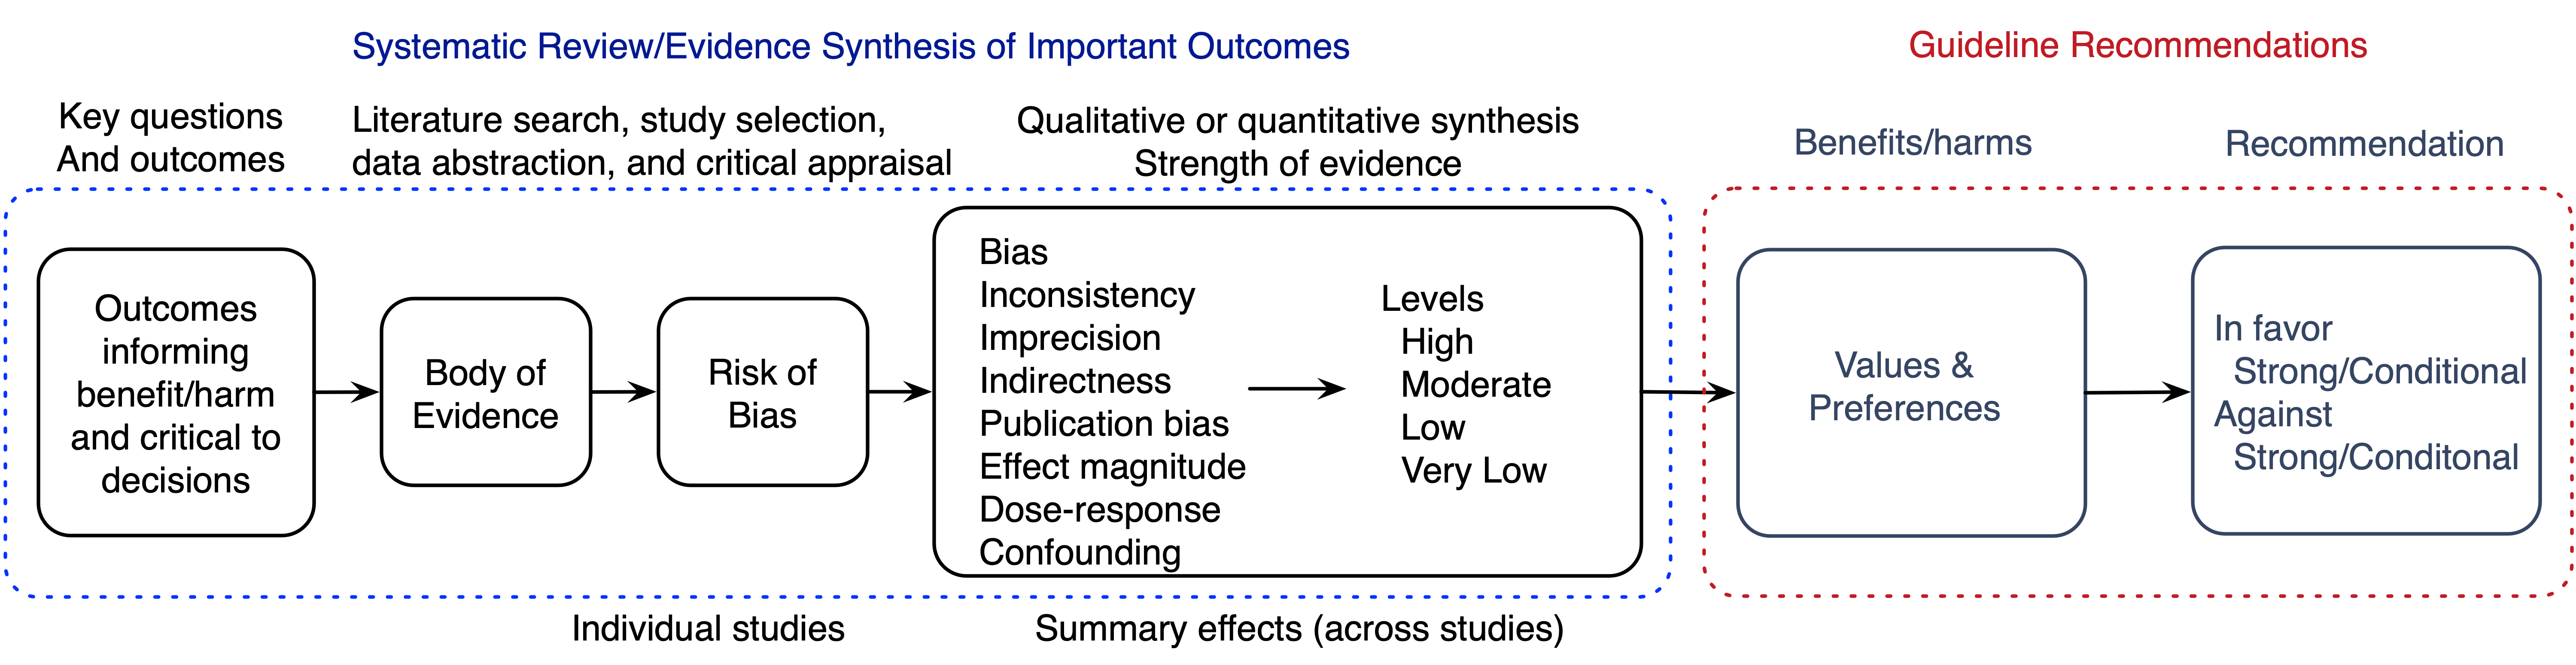
\includegraphics{assets/grade.png}

}

\end{figure}

But ``all models are wrong'' (Box, 1976) --- including GRADE.

\hypertarget{quantitative-synthesis}{%
\section{Quantitative Synthesis}\label{quantitative-synthesis}}

Based on the key question, included studies, clinical and methodological
diversity, results are pooled in either pairwise or network
meta-analyses. Random effects models are fitted given the goal of
estimating unconditional effects (ie, effects not relevant only to the
pooled studies) (Hedges et al., 1998). For binomial outcomes, default
models use the Mantel-Haenszel method; for continuous outcomes inverse
variance weighting. The restricted maximum likelihood estimator is used
to estimate between-study variance (Viechtbauer, 2005). For continuous
or scale-reported outcomes, if means and standard deviations are
unavailable for they are imputed if authors reported medians,
interquartile and/or overall ranges for the effects of interest; and if
necessary P-values are used to estimate missing standard deviations (Shi
et al., 2020). When five or more studies are pooled, the Hartung-Knapp
adjustment is applied (Cornell et al., 2014). Network meta-analyses are
conducted using frequentist (Balduzzi et al., 2023) or Bayesian methods
(Béliveau et al., 2019; Dias et al., 2018) with non-informative priors.
Consistency is examined by comparing direct to indirect evidence in the
frequentist network meta-analyses and inconsistency models in the
Bayesian approach.

Relative effects as reported as risk ratios for clinical
interpretability and continuous outcomes as mean differences or
standardized mean differences for outcomes reported with differing
scales. When feasible, standardized mean differences are re-expressed on
the most common scale used. Statistical heterogeneity is examined using
the between study variance and \emph{I} \(^2\) (Rücker et al., 2008) and
when relevant and practicable explored in subgroup analysis or
meta-regression (Schwarzer et al., 2015; Simon G. Thompson et al., 2002)
Small-study effects and the potential for publication bias are examined
using funnel plots (comparison-adjusted for network meta-analyses),
regression-based tests, and adjustment methods (Balduzzi et al., 2019;
Harrer et al., 2021). Owing to its statistical properties, results using
odds ratios are used reported for when examining small-study effects for
relative effects; sensitivity analyses are performed using risk ratios.

Analyses are conducted using R (R Core Team, 2023) in a reproducible
manner and made publicly available when the practice parameter is
completed.

\hypertarget{harmsadverse-events}{%
\subsection{Harms/Adverse Events}\label{harmsadverse-events}}

Comparative harms are pooled as either relative or absolute effects
according to the frequency of events. For rare events (eg, mortality)
risk differences are most often used.

\hypertarget{selected-analysis-matters}{%
\subsection{Selected Analysis Matters}\label{selected-analysis-matters}}

Age

Surgical classification

The recovery phases described by these tools can be categorised as
early, intermediate and late. The early postoperative recovery phase has
been defined as the first 24 h {[}5, 6{]} or the first seven days
{[}7--9{]}. The speed and extent of recovery in the early phase is
influenced most by pain, nausea, peri-operative medications and delirium
{[}10{]}. The intermediate phase of postoperative recovery has been
defined as the first 28 {[}11{]} or 60 {[}12{]} days. The extent of
recov- ery in the intermediate phase is influenced most by pain, anxiety
and depression, physical impairment and cognitive dysfunction. The late
postoperative recovery phase has been defined as the first six weeks
{[}13{]} or three months {[}14{]}.

\href{https://associationofanaesthetists-publications.onlinelibrary.wiley.com/doi/epdf/10.1111/anae.13312}{Bowyer
2016}

\hypertarget{sensitivity-analyses}{%
\subsection{Sensitivity Analyses}\label{sensitivity-analyses}}

Although useful, meta-analytic results are not without limitations
(Ioannidis, 2016; Maclure et al., 2001) The robustness of meta-analytic
results requires consideration. Aspects include model decisions,
small-study effects, influential studies and other factors (eg, secular
trends, subgroups).

Modeling decisions include the choice of effect measure, estimators, use
of Hartung-Knapp adjustment, continuity corrections for rare events, and
even considering studies without events (can be important for harms). As
relevant, particularly when uncertainty in a pooled effect appears
unclear, how each of these choices impact the range of plausible effects
may be examined.

Small-study effects are particularly important as they may represent
publication bias or selective reporting and can affect the strength of
evidence. \emph{There is, however, no test for publication bias or
selective reporting.} The presence of small-study effects offer clues to
their potential presence, but require a sufficient number of studies
(eg, 10 or more) to effectively examine. Additionally, there are
multiple tests (Begg et al., 1994; Egger et al., 1997; Macaskill et al.,
2001; Peters et al., 2006; Pustejovsky et al., 2019; Sterne et al.,
2011; S. G. Thompson et al., 1999) and adjustment methods --- trim and
fill (Duval et al., 2000), PET-PEESE (Stanley et al., 2014), limit
meta-analyis (Rücker et al., 2011), P-curves (Simonsohn et al., 2014),
and selection models (Copas et al., 2014) that can utilized ---
sometimes offering conflicting results.

We adopt a pragmatic approach to sensitivity analyses. If a pooled
result is obtained from 10 or more studies, the most appropriate choice
of a regression-based test is reported. But if more than one could be
used and results differ both are noted. For adjustment, a limit
meta-analysis is our method of choice superimposed on a funnel plot
(others may be used as sensitivity checks). Although the Hartung-Knapp
adjustment is applied given 5 or more studies, we recognize that
published meta-analyses typically do not. It is therefore important to
understand sensitivity of results to its use and note in the
interpretation of evidence and GRADEing.

Finally, despite the wide range of analytic choices our perspective is
that a convincing body of evidence should not be materially impacted for
a strong recommendation. If it is, then consideration must be
incorporated in both rating the strength of evidence and recommendation.

\hypertarget{rating-the-strength-of-evidence}{%
\section{Rating the Strength of
Evidence}\label{rating-the-strength-of-evidence}}

The strength (certainty) of evidence for important outcomes is appraised
using the Grades of Recommendation, Assessment, Development, and
Evaluation (GRADE Schünemann et al., 2013) and American College of
Cardiology/American Heart Association (ACC/AHA Halperin et al., 2016)
frameworks.

Different conceptual models (Spiegelhalter et al., 2011) underpin these
strength of evidence frameworks --- certainty of evidence (GRADE) and
evidence hierarchy (ACC/AHA). The longstanding evidence hierarchy
(pyramid) model asserts that systematic reviews and meta-analyses of
randomized clinical trials provide the most convincing evidence followed
by randomized clinical trials, observational studies, and case series or
case reports. The certainty of evidence model incorporates the hierarchy
insofar as it reflects study validity, but defines strength of evidence
in terms of how convinced reviewers are that estimates are close to some
``true effect''.

\hypertarget{grade}{%
\subsection{GRADE}\label{grade}}

\hypertarget{tbl-grade-levels}{}
\begin{longtable}[]{@{}
  >{\raggedright\arraybackslash}p{(\columnwidth - 2\tabcolsep) * \real{0.2778}}
  >{\raggedright\arraybackslash}p{(\columnwidth - 2\tabcolsep) * \real{0.7222}}@{}}
\caption{\label{tbl-grade-levels}GRADE levels of
evidence.}\tabularnewline
\toprule\noalign{}
\begin{minipage}[b]{\linewidth}\raggedright
GRADE
\end{minipage} & \begin{minipage}[b]{\linewidth}\raggedright
Definition
\end{minipage} \\
\midrule\noalign{}
\endfirsthead
\toprule\noalign{}
\begin{minipage}[b]{\linewidth}\raggedright
GRADE
\end{minipage} & \begin{minipage}[b]{\linewidth}\raggedright
Definition
\end{minipage} \\
\midrule\noalign{}
\endhead
\bottomrule\noalign{}
\endlastfoot
High & We are very confident that the true effect lies close to that of
the estimate of the effect. \\
Moderate & We are moderately confident in the effect estimate: The true
effect is likely to be close to the estimate of the effect, but there is
a possibility that it is substantially different. \\
Low & Our confidence in the effect estimate is limited: The true effect
may be substantially different from the estimate of the effect. \\
Very low & We have very little confidence in the effect estimate: The
true effect is likely to be substantially different from the estimate of
effect. \\
\end{longtable}

In the GRADE approach, a strength of evidence is determined using an
algorithm that includes limitations in the body of evidence (bias,
inconsistency, imprecision, indirectness, publication bias) and factors
that can increase confidence in effects\footnote{Applies primarily to
  evidence obtained from observational studies.} (large or very large
effect magnitude, dose-response, and plausible residual confounding).
According to study limitations, the strength of evidence may be rated
down 1 or 2 levels according to study limitations from a starting rating
of high for RCTs. Evidence from observational studies begin with a low
rating and may be rated down for limitations or rated up because of
effect magnitude, dose-response, or the impact of plausible residual
confounding. GRADE guidance for rating the certainty of evidence up or
down is followed, with some additions. Inconsistency (unexplained
heterogeneity) of pooled effects is judged by examining statistical
measures (\emph{I} \(^2\) and between-study variance \(\tau^2\))
alongside prediction intervals when there are sufficient studies. Owing
to its well-described limitations, \emph{I} \(^2\) and some
categorization of it's magnitude (eg, small, moderate, or large), is not
used as the primary determinant of heterogeneity (Rücker et al., 2008).
These statistics can vary by effect (associational) measures (eg, risk
vesrus odds ratios and mean versus standardized mean differences) and
are examined for differences in choice.

\begin{figure}

\caption{\label{fig-grading}Process of GRADEing the strength (certainty)
of evidence (after Balshem et al., 2011).}

{\centering 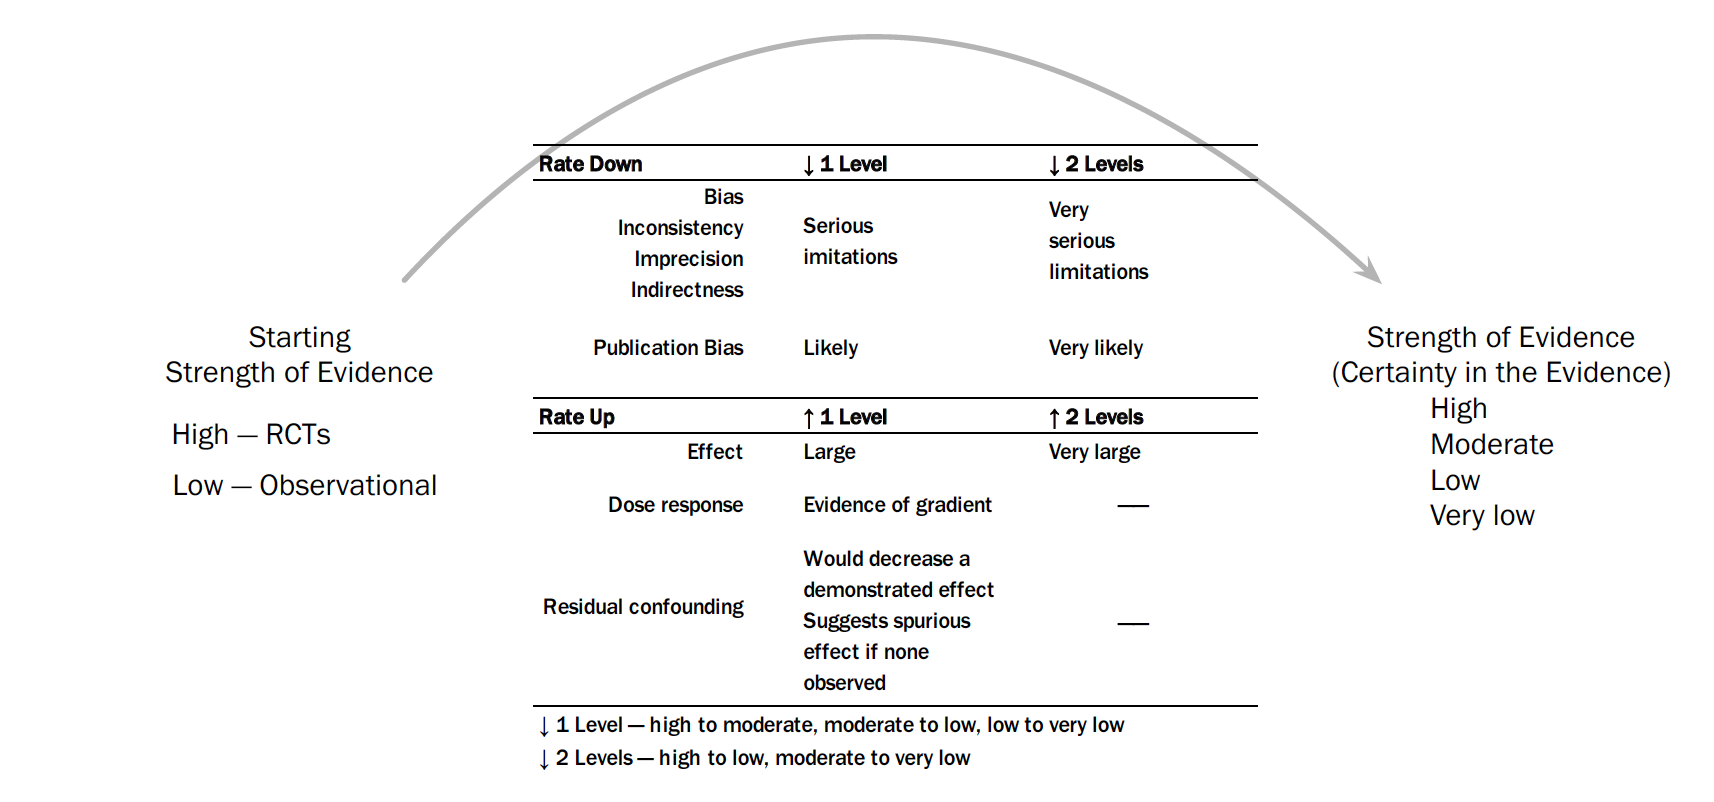
\includegraphics{assets/UpDownGrading.png}

}

\end{figure}

\hypertarget{note-on-nonrandomized-designs-robins-i-and-grade}{%
\subsubsection{Note on Nonrandomized Designs, ROBINS-I, and
GRADE}\label{note-on-nonrandomized-designs-robins-i-and-grade}}

In 2019, the GRADE working group offered ``guidance regarding how
systematic review authors, guideline developers, and health technology
assessment practitioners using GRADE might approach the use of ROBINS-I
as part of the certainty rating process'' (Schünemann et al., 2019).
They suggested that owing to differences in the ROBINS-I tool (referent
to trial emulation) that when it is used, the GRADE for a body of
evidence from non-randomized designs should start at high, not low.
Although a rationale is offered (potential for additional down GRADEing
due to confounding and selection bias), our view is that this guidance
is not appropriate. No matter how careful the conduct and analysis of a
non-randomized design the assumption of no unmeasured confounding is
unverifiable (Schulz et al., 2023) (in stark contrast to randomized
designs). On this basis, it is logically inconsistent to equate
randomized and non-randomized designs. Additionally, the guidance
introduces dependence of GRADE on the risk of bias tool --- absent in
its original formulation. We choose to review carefully our appraisals
of nonrandomized evidence to avoid overzealous down GRADEing, but retain
GRADE in its original formulation.

\hypertarget{comment-on-grade}{%
\subsubsection{Comment on GRADE}\label{comment-on-grade}}

GRADE is complex. The web-based handbook spans over 40,000 words and
there are now over 30 explanatory publications. The 4-level quality of
evidence ratings imposes cutoffs for what is in reality a continuous
scale --- ratings near the cutoffs are less certain than might be
evident. We sometimes struggle assigning a GRADE. Accordingly, the
categorical GRADE (high, moderate, low, very low) reflects in effect the
mode of a distribution. Uncertainty is not conveyed see Llewellyn et al.
(2015) and Stewart et al. (2015).

\hypertarget{accaha}{%
\subsection{ACC/AHA}\label{accaha}}

\hypertarget{tbl-acc-aha}{}
\begin{longtable}[]{@{}
  >{\raggedright\arraybackslash}p{(\columnwidth - 2\tabcolsep) * \real{0.2639}}
  >{\raggedright\arraybackslash}p{(\columnwidth - 2\tabcolsep) * \real{0.7361}}@{}}
\caption{\label{tbl-acc-aha}ACC/AHA levels of evidence.}\tabularnewline
\toprule\noalign{}
\begin{minipage}[b]{\linewidth}\raggedright
Level
\end{minipage} & \begin{minipage}[b]{\linewidth}\raggedright
Definition
\end{minipage} \\
\midrule\noalign{}
\endfirsthead
\toprule\noalign{}
\begin{minipage}[b]{\linewidth}\raggedright
Level
\end{minipage} & \begin{minipage}[b]{\linewidth}\raggedright
Definition
\end{minipage} \\
\midrule\noalign{}
\endhead
\bottomrule\noalign{}
\endlastfoot
A & High-quality evidence from more than 1 RCTs. Meta-analyses of
high-quality RCTs. One or more RCTs corroborated by high-quality
registry studies. \\
B-R & Moderate-quality evidence from 1 or more randomized controlled
trials. Meta-analyses of moderate-quality RCTs. \\
B-NR & Moderate-quality evidence from 1 or more well-designed,
well-executed nonrandomized studies, observational studies, or registry
studies. Meta-analyses of such studies. \\
C-LD & Randomized or nonrandomized observational or registry studies
with limitations of design or execution. Meta-analyses of such studies.
Physiological or mechanistic studies in human subjects. \\
C-EO & Consensus of expert opinion based on clinical experience when
evidence is insufficient, vague, or conflicting. \\
\end{longtable}

RCT: randomized clinical trial; NR: nonrandomized; LD: limited data; EO:
expert opinion

ACC/AHA ratings are based on an evidence hierarchy approach. Its 5-level
scheme (A, B-R, B-NR, C-LD, C-EO) considers study design (RCT,
observational, mechanistic) and quality, number of studies,
meta-analytic results, expert opinion and clinical experience
(Table~\ref{tbl-acc-aha}). The framework explicitly allows for
consideration of mechanistic studies conducted in humans (Goodman et
al., 2013). Unlike GRADE guidance for arriving at a strength of evidence
is limited to the level of evidence definitions. The ratings were
recently revised from an A, B, C scheme by expanding B and C into 2
subcategories and adding E for expert opinion (A. K. Jacobs et al.,
2014).

\bookmarksetup{startatroot}

\hypertarget{recommendations}{%
\chapter{Recommendations}\label{recommendations}}

\hypertarget{formulating-recommendations}{%
\section{Formulating
Recommendations}\label{formulating-recommendations}}

Language

Formula

\hypertarget{strength-of-recommendations}{%
\section{Strength of
Recommendations}\label{strength-of-recommendations}}

The categories of recommendations in the GRADE approach include strong
in favor, weak in favor, weak against, and strong against an
intervention. Strong recommendations reflect Task Force believing all or
almost all clinicians would choose the specific action or approach. Weak
recommendations are those where most, but not all, would choose the
action or approach.

The categories of recommendations in the GRADE approach include: strong
in favor, weak in favor, weak against, and strong against
(Table\textasciitilde{}\ref{tab:sor}) \cite{Andrews2013}. Strong
recommendations reflect authors believing all or almost all clinicians
would choose the specific action or approach. Weak recommendations are
those where most, but not all, would choose the action or approach.
Although not included in the formal GRADE guidance, its developers
recommend guideline panels distinguish good or best practice statements
from guideline recommendations. Good practice statements are those where
evidence is inappropriate for a strength of evidence rating
\cite{Guyatt2015,Guyatt2016}. An example where best practice statements
are included in addition to the GRADEd ones is the 2016 Surviving Sepsis
Campaign guidelines \cite{Rhodes2017}.

ACC/AHA \soe~ratings are based on an evidence hierarchy approach. Its
5-level \soe~rating scheme (A, B-R, B-NR, C-LD, C-EO) considers study
design (RCT, observational, mechanistic) and quality, number of studies,
meta-analytic results, expert opinion and clinical experience
(Table\textasciitilde{}\ref{tab:soe}, Appendix
Figure\textasciitilde{}\ref{fig:appendix_acc}).\\
Recent guidelines \cite{Reboussin2018} have used the Cochrane risk of
bias tool to appraise individual studies, but an ACCF/AHA Evidence
Grading Tool is apparently under development \cite{Jacobs2013}. The
framework explicitly allows for consideration of mechanistic studies
\cite{Goodman2013} conducted in humans. Unlike GRADE and AHRQ/USPSTF
approaches, guidance for arriving at a \soe~is limited to the level of
evidence definitions. The ratings were recently revised from an A, B, C
scheme by expanding B and C into 2 subcategories and adding E for expert
opinion \cite{Jacobs2014}.

\hypertarget{best-practice-statements}{%
\section{Best Practice Statements}\label{best-practice-statements}}

\hypertarget{no-recommendation}{%
\section{No Recommendation}\label{no-recommendation}}

\hypertarget{soe-sor-discordance}{%
\section{SOE SOR Discordance}\label{soe-sor-discordance}}

\bookmarksetup{startatroot}

\hypertarget{support-external-guidance}{%
\chapter{Support -- External Guidance}\label{support-external-guidance}}

Guidance documents submitted by external organizations for support from
the ASA are reviewed by the CPP and a committee with content expertise.
Support is offered in 3 categories:

\begin{enumerate}
\def\labelenumi{\arabic{enumi}.}
\item
  \textbf{Endorsement} --- The document should generally satisfy ASA's
  guideline development requirements and there is general agreement with
  all recommendations in the document. Guidance developed with an
  official representative from the ASA and approved through governance
  procedures are considered in this category.
\item
  \textbf{Affirmation of Value} --- External organization's guidelines
  or practice parameters that have merit and value but either do not
  generally satisfy ASA's guideline development requirements or there is
  not general agreement with all recommendations in the document.
  Statements and policy papers may be considered for affirmation of
  value.
\item
  \textbf{No Endorsement or Affirmation of Value} --- The external
  organization's document does not meet ASA guideline development
  requirements and is not felt to be of benefit to the ASA membership.
\end{enumerate}

Although a complete description of the process for determining the
category of support is beyond the scope here, the review conducted by
the methodologists is outlined as it is an important function.

An objective methodological review of approaches used in developing
guidance facilitates endorsement decisions. The purpose of the
methodological review is not to offer a judgment on whether the guidance
document should be endorsed or supported, but to provide a sufficiently
detailed appraisal of the methods to allow informed decisions according
to the administrative procedures.

The methodological review includes two main sections:

\begin{enumerate}
\def\labelenumi{\arabic{enumi}.}
\tightlist
\item
  Appraisal of conforming to standards for systematic review conduct
  (Eden, 2011) and developing recommendations (Graham, 2011) using the
  NEATS (Jue et al., 2019) tool (National Guideline Clearinghouse Extent
  of Adherence to Trustworthy Standards) for practice guidelines and
  AGREE-II (Brouwers et al., 2016) modified (C. Jacobs et al., 2014) for
  consensus statements.
\item
  A narrative description of the limitations and strengths from a
  methodological perspective.
\end{enumerate}

Depending on the scope and complexity, reviews are conducted by one or
two methodologists.

Examples of the NEATS and modified AGREE-II appraisals

\begin{figure}

\caption{\label{fig-neats}Example of NEATS appraisal.}

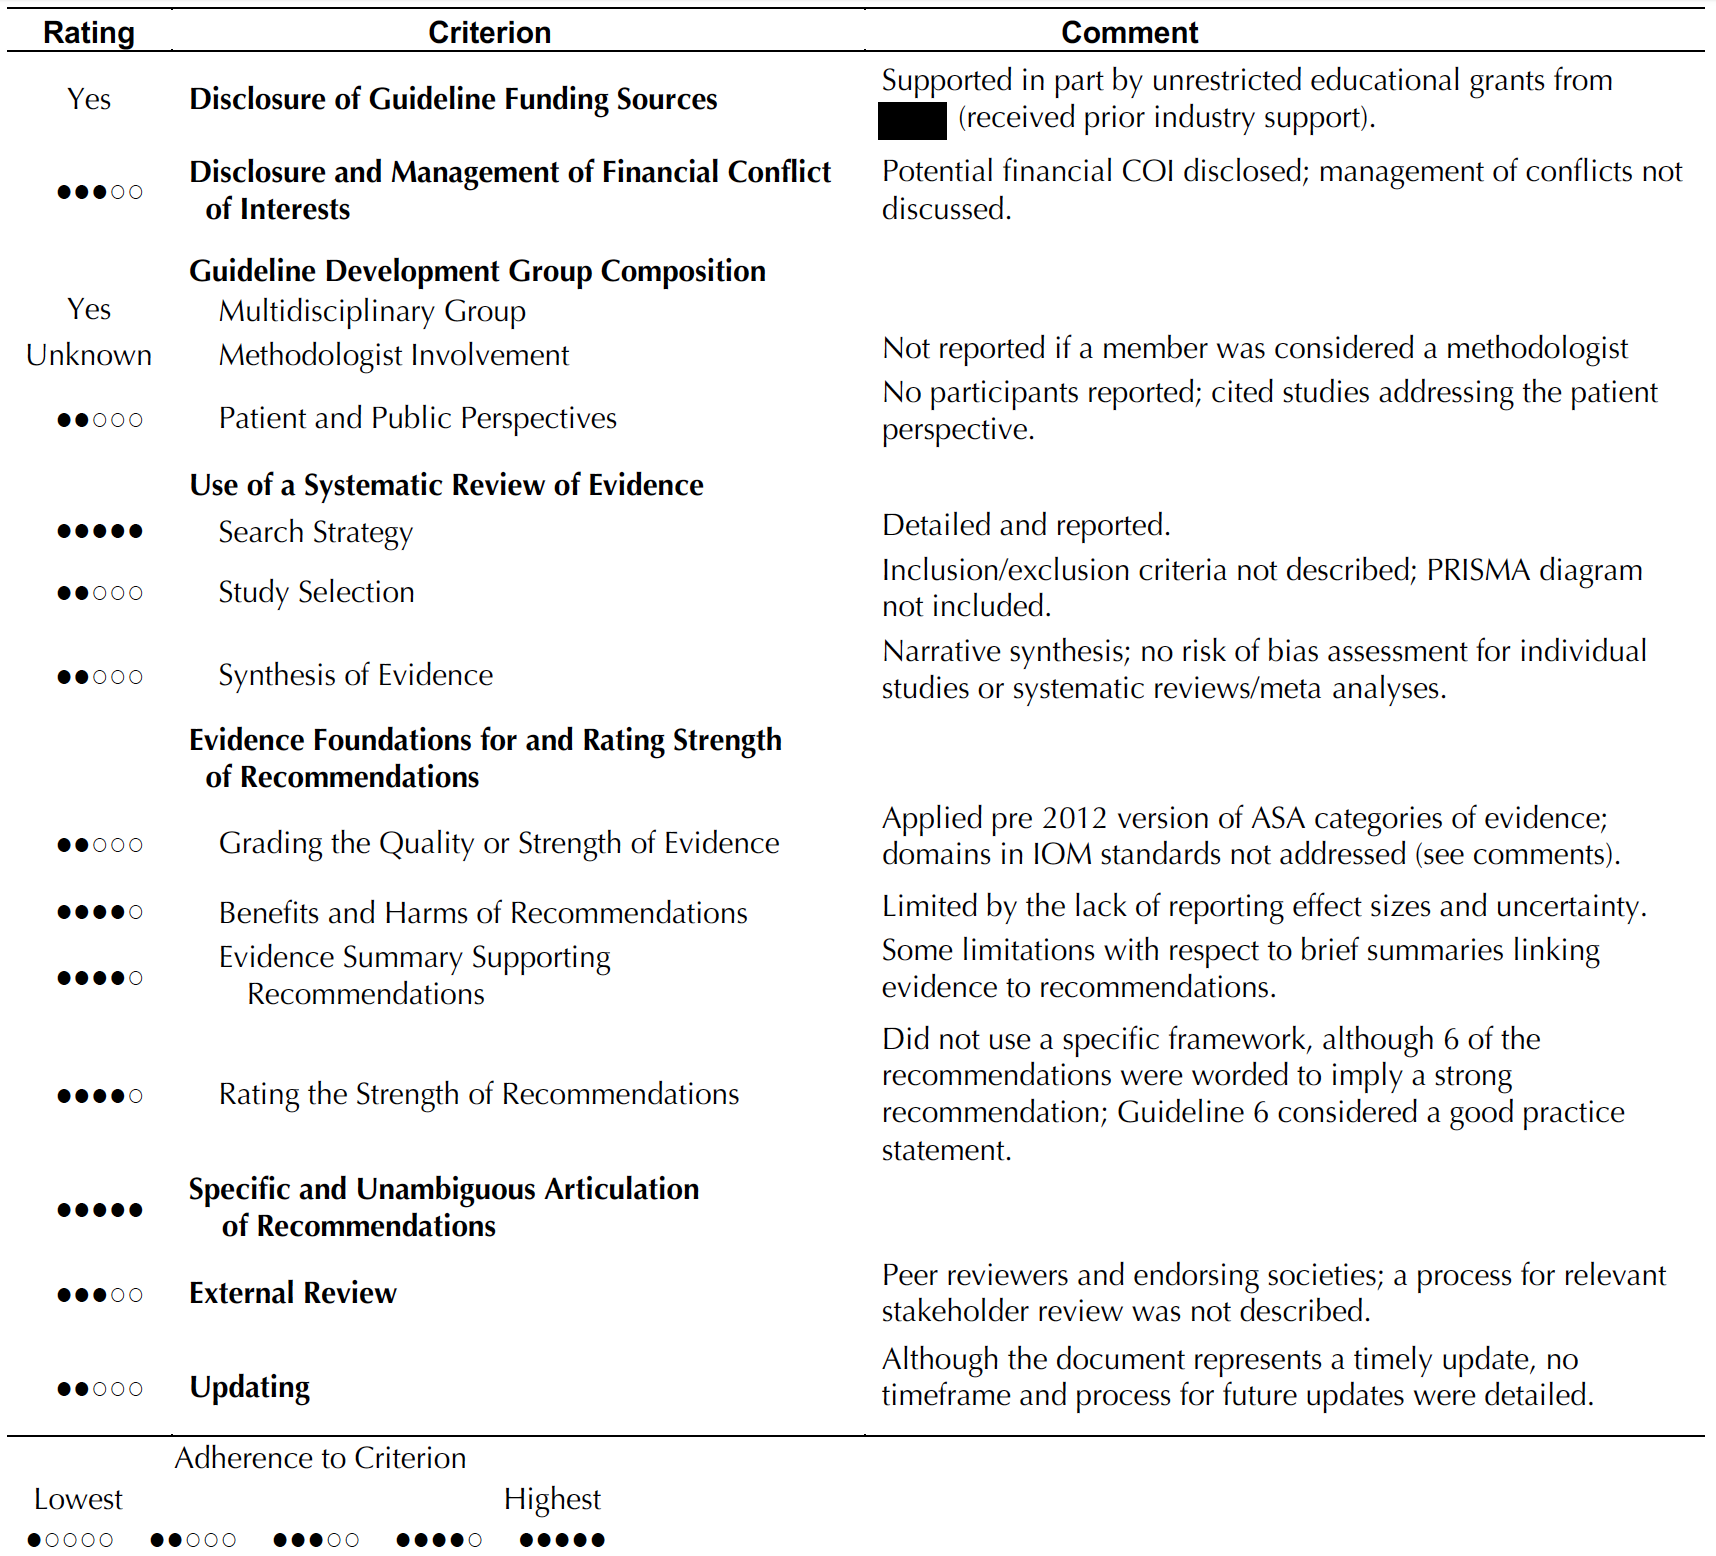
\includegraphics[width=0.9\textwidth,height=\textheight]{assets/neatsExample.png} \hfill{}

\end{figure}

\begin{figure}

\caption{\label{fig-agree}Example of modified AGREE-II appraisal.}

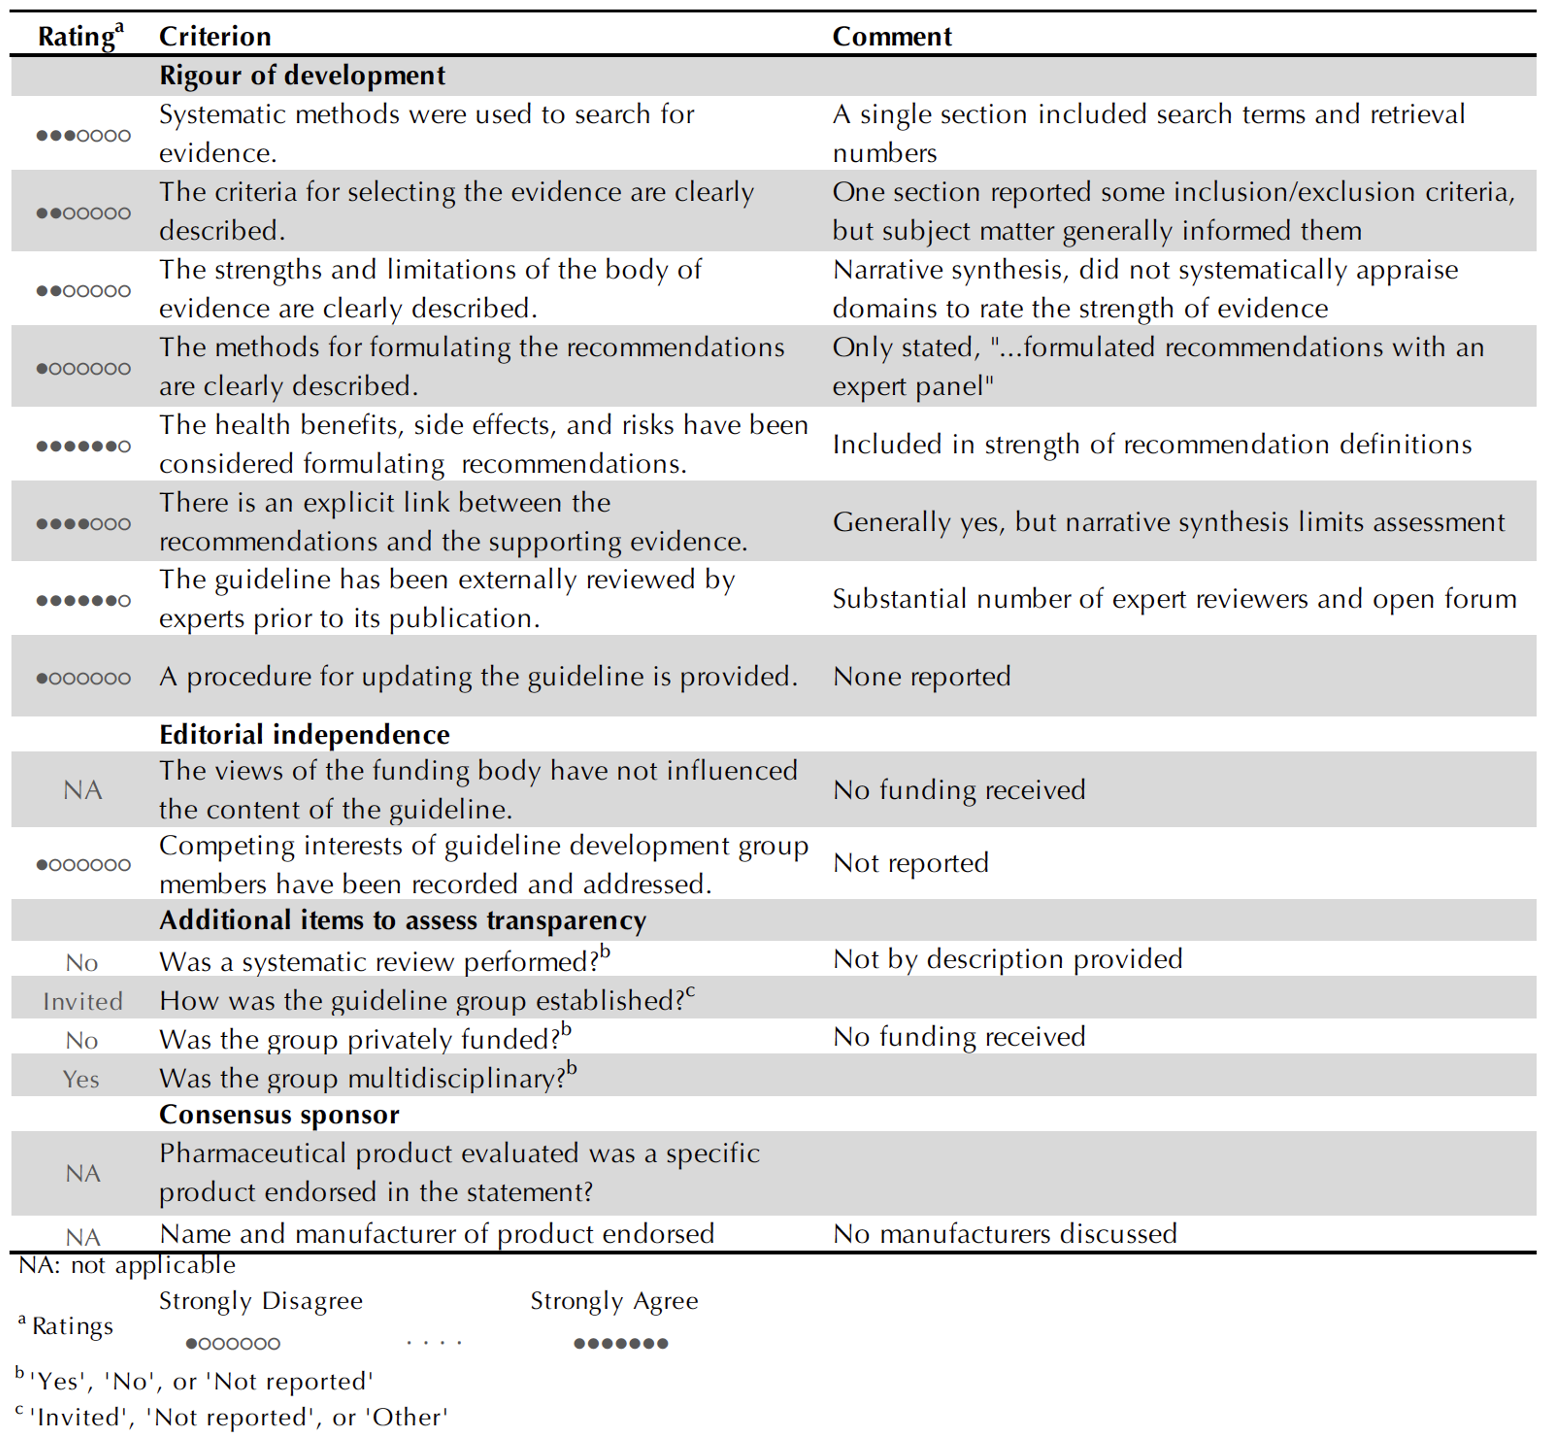
\includegraphics[width=0.9\textwidth,height=\textheight]{assets/agreeExample.png} \hfill{}

\end{figure}

\bookmarksetup{startatroot}

\hypertarget{summary}{%
\chapter{Summary}\label{summary}}

\bookmarksetup{startatroot}

\hypertarget{references}{%
\chapter*{References}\label{references}}
\addcontentsline{toc}{chapter}{References}

\markboth{References}{References}

\hypertarget{refs}{}
\begin{CSLReferences}{1}{0}
\leavevmode\vadjust pre{\hypertarget{ref-Balduzzi2023}{}}%
Balduzzi, S., Rücker, G., Nikolakopoulou, A., Papakonstantinou, T.,
Salanti, G., Efthimiou, O., \& Schwarzer, G. (2023). Netmeta: An r
package for network meta-analysis using frequentist methods.
\emph{Journal of Statistical Software}, \emph{106}, 1--40.

\leavevmode\vadjust pre{\hypertarget{ref-Balduzzi2019}{}}%
Balduzzi, S., Rücker, G., \& Schwarzer, G. (2019). How to perform a
meta-analysis with r: A practical tutorial. \emph{BMJ Ment Health},
\emph{22}(4), 153--160.

\leavevmode\vadjust pre{\hypertarget{ref-Balshem2011}{}}%
Balshem, H., Helfand, M., Schunemann, H. J., Oxman, A. D., Kunz, R.,
Brozek, J., Vist, G. E., Falck-Ytter, Y., Meerpohl, J., Norris, S., \&
Guyatt, G. H. (2011). GRADE guidelines: 3. Rating the quality of
evidence {[}Journal Article{]}. \emph{J Clin Epidemiol}, \emph{64}(4),
401--406. doi:
\href{https://doi.org/10.1016/j.jclinepi.2010.07.015}{10.1016/j.jclinepi.2010.07.015}

\leavevmode\vadjust pre{\hypertarget{ref-Begg1994}{}}%
Begg, C. B., \& Mazumdar, M. (1994).
\href{https://www.ncbi.nlm.nih.gov/pubmed/7786990}{Operating
characteristics of a rank correlation test for publication bias}.
\emph{Biometrics}, \emph{50}(4), 1088--1101.

\leavevmode\vadjust pre{\hypertarget{ref-Beliveau2019}{}}%
Béliveau, A., Boyne, D. J., Slater, J., Brenner, D., \& Arora, P.
(2019). BUGSnet: An r package to facilitate the conduct and reporting of
bayesian network meta-analyses. \emph{BMC Med Res Methodol},
\emph{19}(1), 196. doi:
\href{https://doi.org/10.1186/s12874-019-0829-2}{10.1186/s12874-019-0829-2}

\leavevmode\vadjust pre{\hypertarget{ref-Booth2012}{}}%
Booth, A., Clarke, M., Dooley, G., Ghersi, D., Moher, D., Petticrew, M.,
\& Stewart, L. (2012). The nuts and bolts of PROSPERO: An international
prospective register of systematic reviews. \emph{Syst Rev}, \emph{1},
2. doi:
\href{https://doi.org/10.1186/2046-4053-1-2}{10.1186/2046-4053-1-2}

\leavevmode\vadjust pre{\hypertarget{ref-Box1976}{}}%
Box, G. E. (1976). Science and statistics. \emph{Journal of the American
Statistical Association}, \emph{71}(356), 791--799.

\leavevmode\vadjust pre{\hypertarget{ref-Brouwers2016}{}}%
Brouwers, M. C., Kerkvliet, K., Spithoff, K., \& AGREE Next Steps
Consortium. (2016). The {AGREE} reporting checklist: A tool to improve
reporting of clinical practice guidelines. \emph{BMJ}, \emph{352},
i1152. doi: \href{https://doi.org/10.1136/bmj.i1152}{10.1136/bmj.i1152}

\leavevmode\vadjust pre{\hypertarget{ref-Caplan1993}{}}%
Caplan, R. A., Benumof, J. L., Berry, F. A., Blitt, C. D., Bode, R. H.,
Cheney, F. W., Connis, R. T., Guidry, O. F., \& Ovassapian, A. (1993).
Practice guidelines for management of the difficult airway. A report by
the american society of anesthesiologists task force on management of
the difficult airway. \emph{Anesthesiology}, \emph{78}(3), 597--602.

\leavevmode\vadjust pre{\hypertarget{ref-Copas2014}{}}%
Copas, J., Dwan, K., Kirkham, J., \& Williamson, P. (2014). A
model-based correction for outcome reporting bias in meta-analysis.
\emph{Biostatistics}, \emph{15}(2), 370--383. doi:
\href{https://doi.org/10.1093/biostatistics/kxt046}{10.1093/biostatistics/kxt046}

\leavevmode\vadjust pre{\hypertarget{ref-Cornell2014}{}}%
Cornell, J. E., Mulrow, C. D., Localio, R., Stack, C. B., Meibohm, A.
R., Guallar, E., \& Goodman, S. N. (2014). Random-effects meta-analysis
of inconsistent effects: A time for change. \emph{Ann Intern Med},
\emph{160}(4), 267--270. doi:
\href{https://doi.org/10.7326/M13-2886}{10.7326/M13-2886}

\leavevmode\vadjust pre{\hypertarget{ref-Dias2018a}{}}%
Dias, S., Ades, A. E., Welton, N. J., Jansen, J. P., \& Sutton, A. J.
(2018). \emph{Network meta-analysis for decision-making}. John Wiley \&
Sons.

\leavevmode\vadjust pre{\hypertarget{ref-Duval2000}{}}%
Duval, S., \& Tweedie, R. (2000). Trim and fill: A simple
funnel-plot-based method of testing and adjusting for publication bias
in meta-analysis. \emph{Biometrics}, \emph{56}(2), 455--463. doi:
\href{https://doi.org/10.1111/j.0006-341x.2000.00455.x}{10.1111/j.0006-341x.2000.00455.x}

\leavevmode\vadjust pre{\hypertarget{ref-Eden2011}{}}%
Eden, J. (2011). \emph{Finding what works in health care: Standards for
systematic reviews}. Washington, D.C.: National Academies Press.

\leavevmode\vadjust pre{\hypertarget{ref-Egger1997}{}}%
Egger, M., Zellweger-Zähner, T., Schneider, M., Junker, C., Lengeler,
C., \& Antes, G. (1997). Language bias in randomised controlled trials
published in english and german. \emph{Lancet}, \emph{350}(9074),
326--329. doi:
\href{https://doi.org/10.1016/S0140-6736(97)02419-7}{10.1016/S0140-6736(97)02419-7}

\leavevmode\vadjust pre{\hypertarget{ref-Goodman2013}{}}%
Goodman, S. N., \& Gerson, J. (2013).
\href{https://www.ncbi.nlm.nih.gov/pubmed/24027800}{Mechanistic evidence
in evidence-based medicine: A conceptual framework}. In AHRQ Methods for
Effective Health Care. AHRQ Methods for Effective Health Care, Agency
for Healthcare Research; Quality (US), Rockville (MD).

\leavevmode\vadjust pre{\hypertarget{ref-Graham2011}{}}%
Graham, R. (2011). \emph{Clinical practice guidelines we can trust}.
Washington, DC: National Academies Press.

\leavevmode\vadjust pre{\hypertarget{ref-Guyatt2011}{}}%
Guyatt, G. H., Oxman, A. D., Kunz, R., Atkins, D., Brozek, J., Vist, G.,
Alderson, P., Glasziou, P., Falck-Ytter, Y., \& Schunemann, H. J.
(2011). GRADE guidelines: 2. Framing the question and deciding on
important outcomes. \emph{J Clin Epidemiol}, \emph{64}(4), 395--400.
doi:
\href{https://doi.org/10.1016/j.jclinepi.2010.09.012}{10.1016/j.jclinepi.2010.09.012}

\leavevmode\vadjust pre{\hypertarget{ref-Haddaway2022}{}}%
Haddaway, N. R., Grainger, M. J., \& Gray, C. T. (2022). Citationchaser:
A tool for transparent and efficient forward and backward citation
chasing in systematic searching. \emph{Res Synth Methods}, \emph{13}(4),
533--545. doi:
\href{https://doi.org/10.1002/jrsm.1563}{10.1002/jrsm.1563}

\leavevmode\vadjust pre{\hypertarget{ref-Halperin2016}{}}%
Halperin, J. L., Levine, G. N., Al-Khatib, S. M., Birtcher, K. K.,
Bozkurt, B., Brindis, R. G., Cigarroa, J. E., Curtis, L. H., Fleisher,
L. A., Gentile, F., Gidding, S., Hlatky, M. A., Ikonomidis, J., Joglar,
J., Pressler, S. J., \& Wijeysundera, D. N. (2016). Further evolution of
the ACC/AHA clinical practice guideline recommendation classification
system: A report of the american college of cardiology/american heart
association task force on clinical practice guidelines. \emph{J Am Coll
Cardiol}, \emph{67}(13), 1572--1574. doi:
\href{https://doi.org/10.1016/j.jacc.2015.09.001}{10.1016/j.jacc.2015.09.001}

\leavevmode\vadjust pre{\hypertarget{ref-Harrer2021}{}}%
Harrer, M., Cuijpers, P., Furukawa, T., \& Ebert, D. (2021). \emph{Doing
meta-analysis with r: A hands-on guide}. Chapman; Hall/CRC.

\leavevmode\vadjust pre{\hypertarget{ref-House1990}{}}%
Health Subcommittee Hearing. (1990). \emph{Hearing before the
subcommittee on health of the committee on ways and means house of
representatives one hundred first congress second session april 23, 1990
serial 101-95}.

\leavevmode\vadjust pre{\hypertarget{ref-Hedges1998}{}}%
Hedges, L. V., \& Vevea, J. L. (1998). Fixed-and random-effects models
in meta-analysis. \emph{Psychological Methods}, \emph{3}(4), 486. doi:
\url{http://dx.doi.org/10.1037/1082-989X.3.4.486}

\leavevmode\vadjust pre{\hypertarget{ref-Ioannidis2016}{}}%
Ioannidis, J. P. A. (2016). The mass production of redundant,
misleading, and conflicted systematic reviews and meta-analyses.
\emph{Milbank Q}, \emph{94}(3), 485--514. doi:
\href{https://doi.org/10.1111/1468-0009.12210}{10.1111/1468-0009.12210}

\leavevmode\vadjust pre{\hypertarget{ref-Jacobs2014}{}}%
Jacobs, A. K., Anderson, J. L., \& Halperin, J. L. (2014). The evolution
and future of {ACC/AHA} clinical practice guidelines: A 30-year journey:
A report of the {American College of Cardiology/American Heart
Association Task Force on Practice Guidelines}. \emph{J Am Coll
Cardiol}, \emph{64}(13), 1373--1384. doi:
\href{https://doi.org/10.1016/j.jacc.2014.06.001}{10.1016/j.jacc.2014.06.001}

\leavevmode\vadjust pre{\hypertarget{ref-Jacobs2014a}{}}%
Jacobs, C., Graham, I. D., Makarski, J., Chassé, M., Fergusson, D.,
Hutton, B., \& Clemons, M. (2014). Clinical practice guidelines and
consensus statements in oncology--an assessment of their methodological
quality. \emph{PLoS One}, \emph{9}(10), e110469. doi:
\href{https://doi.org/10.1371/journal.pone.0110469}{10.1371/journal.pone.0110469}

\leavevmode\vadjust pre{\hypertarget{ref-Jia2020}{}}%
Jia, Y., Huang, D., Wen, J., Wang, Y., Rosman, L., Chen, Q., Robinson,
K. A., Gagnier, J. J., Ehrhardt, S., \& Celentano, D. D. (2020).
Assessment of language and indexing biases among chinese-sponsored
randomized clinical trials. \emph{JAMA Netw Open}, \emph{3}(5), e205894.
doi:
\href{https://doi.org/10.1001/jamanetworkopen.2020.5894}{10.1001/jamanetworkopen.2020.5894}

\leavevmode\vadjust pre{\hypertarget{ref-Jue2019}{}}%
Jue, J. J., Cunningham, S., Lohr, K., Shekelle, P., Shiffman, R.,
Robbins, C., Nix, M., Coates, V., \& Schoelles, K. (2019). Developing
and testing the agency for healthcare research and quality's national
guideline clearinghouse extent of adherence to trustworthy standards
(NEATS) instrument. \emph{Ann Intern Med}, \emph{170}(7), 480--487. doi:
\href{https://doi.org/10.7326/M18-2950}{10.7326/M18-2950}

\leavevmode\vadjust pre{\hypertarget{ref-Juni2002}{}}%
Jüni, P., Holenstein, F., Sterne, J., Bartlett, C., \& Egger, M. (2002).
Direction and impact of language bias in meta-analyses of controlled
trials: Empirical study. \emph{Int J Epidemiol}, \emph{31}(1), 115--123.
doi: \href{https://doi.org/10.1093/ije/31.1.115}{10.1093/ije/31.1.115}

\leavevmode\vadjust pre{\hypertarget{ref-Llewellyn2015}{}}%
Llewellyn, A., Whittington, C., Stewart, G., Higgins, J. P., \& Meader,
N. (2015). The use of {Bayesian} networks to assess the quality of
evidence from research synthesis: 2. {I}nter-rater reliability and
comparison with standard {GRADE} assessment. \emph{PLoS One},
\emph{10}(12), e0123511. doi:
\href{https://doi.org/10.1371/journal.pone.0123511}{10.1371/journal.pone.0123511}

\leavevmode\vadjust pre{\hypertarget{ref-Macaskill2001}{}}%
Macaskill, P., Walter, S. D., \& Irwig, L. (2001). A comparison of
methods to detect publication bias in meta-analysis. \emph{Stat Med},
\emph{20}(4), 641--654. doi:
\href{https://doi.org/10.1002/sim.698}{10.1002/sim.698}

\leavevmode\vadjust pre{\hypertarget{ref-Maclure2001}{}}%
Maclure, M., \& Schneeweiss, S. (2001). Causation of bias: The episcope.
\emph{Epidemiology}, \emph{12}(1), 114--122. doi:
\href{https://doi.org/10.1097/00001648-200101000-00019}{10.1097/00001648-200101000-00019}

\leavevmode\vadjust pre{\hypertarget{ref-Mao2020}{}}%
Mao, C., \& Li, M. (2020). Language bias among chinese-sponsored
randomized clinical trials in systematic reviews and meta-analyses-can
anything be done? \emph{JAMA Netw Open}, \emph{3}(5), e206370. doi:
\href{https://doi.org/10.1001/jamanetworkopen.2020.6370}{10.1001/jamanetworkopen.2020.6370}

\leavevmode\vadjust pre{\hypertarget{ref-Meltzer2011}{}}%
Meltzer, D. O., Hoomans, T., Chung, J. W., \& Basu, A. (2011). Minimal
modeling approaches to value of information analysis for health
research. \emph{Med Decis Making}, \emph{31}(6), E1--E22. doi:
\href{https://doi.org/10.1177/0272989X11412975}{10.1177/0272989X11412975}

\leavevmode\vadjust pre{\hypertarget{ref-Pallath2023}{}}%
Pallath, A., \& Zhang, Q. (2023). Paperfetcher: A tool to automate
handsearching and citation searching for systematic reviews. \emph{Res
Synth Methods}, \emph{14}(2), 323--335. doi:
\href{https://doi.org/10.1002/jrsm.1604}{10.1002/jrsm.1604}

\leavevmode\vadjust pre{\hypertarget{ref-PCORI2019}{}}%
PCORI. (2019). \emph{Patient-centered outcomes research institute
methodology standards 11: Standards for systematic reviews.} {PCORI}.
Retrieved from
\url{https://www.pcori.org/research/about-our-research/research-methodology/pcori-methodology-standards\#Systematic\%20Reviews}

\leavevmode\vadjust pre{\hypertarget{ref-Peters2006}{}}%
Peters, J. L., Sutton, A. J., Jones, D. R., Abrams, K. R., \& Rushton,
L. (2006). Comparison of two methods to detect publication bias in
meta-analysis. \emph{JAMA}, \emph{295}(6), 676--680. doi:
\href{https://doi.org/10.1001/jama.295.6.676}{10.1001/jama.295.6.676}

\leavevmode\vadjust pre{\hypertarget{ref-Polanin2019}{}}%
Polanin, J. R., Pigott, T. D., Espelage, D. L., \& Grotpeter, J. K.
(2019). Best practice guidelines for abstract screening large‐evidence
systematic reviews and meta‐analyses. \emph{Research Synthesis Methods},
\emph{10}(3), 330--342. Retrieved from
\url{http://europepmc.org/abstract/PMC/PMC6771536}

\leavevmode\vadjust pre{\hypertarget{ref-Pustejovsky2019}{}}%
Pustejovsky, J. E., \& Rodgers, M. A. (2019). Testing for funnel plot
asymmetry of standardized mean differences. \emph{Res Synth Methods},
\emph{10}(1), 57--71. doi:
\href{https://doi.org/10.1002/jrsm.1332}{10.1002/jrsm.1332}

\leavevmode\vadjust pre{\hypertarget{ref-R2023}{}}%
R Core Team. (2023). \emph{R: A language and environment for statistical
computing}. Vienna, Austria: R Foundation for Statistical Computing.
Retrieved from \url{https://www.R-project.org/}

\leavevmode\vadjust pre{\hypertarget{ref-Roizen1993}{}}%
Roizen, M. F., Berger, D. I., Gabel, R. A., Gerson, J., Mark, J. B.,
Parks, R. I., Paulus, D. A., Smith, J. S., \& Woolf, S. H. (1993).
Practice guidelines for pulmonary artery catheterization. A report by
the american society of anesthesiologists task force on pulmonary artery
catheterization. \emph{Anesthesiology}, \emph{78}(2), 380--394.

\leavevmode\vadjust pre{\hypertarget{ref-Rucker2011}{}}%
Rücker, G., Schwarzer, G., Carpenter, J. R., Binder, H., \& Schumacher,
M. (2011). Treatment-effect estimates adjusted for small-study effects
via a limit meta-analysis. \emph{Biostatistics}, \emph{12}(1), 122--142.
doi:
\href{https://doi.org/10.1093/biostatistics/kxq046}{10.1093/biostatistics/kxq046}

\leavevmode\vadjust pre{\hypertarget{ref-Rucker2008}{}}%
Rücker, G., Schwarzer, G., Carpenter, J. R., \& Schumacher, M. (2008).
Undue reliance on {I}\(^2\) in assessing heterogeneity may mislead.
\emph{BMC Med Res Methodol}, \emph{8}, 79. doi:
\href{https://doi.org/10.1186/1471-2288-8-79}{10.1186/1471-2288-8-79}

\leavevmode\vadjust pre{\hypertarget{ref-Schulz2023}{}}%
Schulz, J., Moodie, E. E. M., \& Shortreed, S. M. (2023). NO UNMEASURED
CONFOUNDING: KNOWN UNKNOWNS OR{\ldots{}} NOT? \emph{Am J Epidemiol},
\emph{192}(9), 1604--1605. doi:
\href{https://doi.org/10.1093/aje/kwad133}{10.1093/aje/kwad133}

\leavevmode\vadjust pre{\hypertarget{ref-GRADE}{}}%
Schünemann, H., Broz̀ek, J., Guyatt, G., \& Oxman, A. (2013).
\emph{{GRADE Handbook}}. Retrieved from
\url{https://gdt.gradepro.org/app/handbook/handbook.html}

\leavevmode\vadjust pre{\hypertarget{ref-Schunemann2019}{}}%
Schünemann, H., Cuello, C., Akl, E. A., Mustafa, R. A., Meerpohl, J. J.,
Thayer, K., Morgan, R. L., Gartlehner, G., Kunz, R., Katikireddi, S. V.,
Sterne, J., Higgins, J. P., Guyatt, G., \& GRADE Working Group. (2019).
GRADE guidelines: 18. How ROBINS-i and other tools to assess risk of
bias in nonrandomized studies should be used to rate the certainty of a
body of evidence. \emph{J Clin Epidemiol}, \emph{111}, 105--114. doi:
\href{https://doi.org/10.1016/j.jclinepi.2018.01.012}{10.1016/j.jclinepi.2018.01.012}

\leavevmode\vadjust pre{\hypertarget{ref-Schwarzer2015}{}}%
Schwarzer, G., Carpenter, J. R., \& Rücker, G. (2015).
\emph{Meta-analysis with {R}}. Springer.

\leavevmode\vadjust pre{\hypertarget{ref-Shi2020}{}}%
Shi, J., Luo, D., Weng, H., Zeng, X.-T., Lin, L., Chu, H., \& Tong, T.
(2020). Optimally estimating the sample standard deviation from the
five-number summary. \emph{Res Synth Methods}, \emph{11}(5), 641--654.
doi: \href{https://doi.org/10.1002/jrsm.1429}{10.1002/jrsm.1429}

\leavevmode\vadjust pre{\hypertarget{ref-Simonsohn2014}{}}%
Simonsohn, U., Nelson, L. D., \& Simmons, J. P. (2014). P-curve and
effect size: Correcting for publication bias using only significant
results. \emph{Perspect Psychol Sci}, \emph{9}(6), 666--681. doi:
\href{https://doi.org/10.1177/1745691614553988}{10.1177/1745691614553988}

\leavevmode\vadjust pre{\hypertarget{ref-Spiegelhalter2004}{}}%
Spiegelhalter, D. J., Abrams, K. R., \& Myles, J. P. (2004).
\emph{Bayesian approaches to clinical trials and health care
evaluation}. Wiley.

\leavevmode\vadjust pre{\hypertarget{ref-Spiegelhalter2011}{}}%
Spiegelhalter, D. J., \& Riesch, H. (2011). Don't know, can't know:
Embracing deeper uncertainties when analysing risks. \emph{Philos Trans
A Math Phys Eng Sci}, \emph{369}(1956), 4730--4750. doi:
\href{https://doi.org/10.1098/rsta.2011.0163}{10.1098/rsta.2011.0163}

\leavevmode\vadjust pre{\hypertarget{ref-Stanley2014}{}}%
Stanley, T. D., \& Doucouliagos, H. (2014). Meta-regression
approximations to reduce publication selection bias. \emph{Res Synth
Methods}, \emph{5}(1), 60--78. doi:
\href{https://doi.org/10.1002/jrsm.1095}{10.1002/jrsm.1095}

\leavevmode\vadjust pre{\hypertarget{ref-Sterne2011}{}}%
Sterne, J. A. C., Sutton, A. J., Ioannidis, J. P. A., Terrin, N., Jones,
D. R., Lau, J., Carpenter, J., Rücker, G., Harbord, R. M., Schmid, C.
H., Tetzlaff, J., Deeks, J. J., Peters, J., Macaskill, P., Schwarzer,
G., Duval, S., Altman, D. G., Moher, D., \& Higgins, J. P. T. (2011).
Recommendations for examining and interpreting funnel plot asymmetry in
meta-analyses of randomised controlled trials. \emph{BMJ}, \emph{343},
d4002. doi: \href{https://doi.org/10.1136/bmj.d4002}{10.1136/bmj.d4002}

\leavevmode\vadjust pre{\hypertarget{ref-Stewart2015}{}}%
Stewart, G. B., Higgins, J. P. T., Schünemann, H., \& Meader, N. (2015).
The use of bayesian networks to assess the quality of evidence from
research synthesis: 1. \emph{PLoS One}, \emph{10}(3), e0114497. doi:
\href{https://doi.org/10.1371/journal.pone.0114497}{10.1371/journal.pone.0114497}

\leavevmode\vadjust pre{\hypertarget{ref-Thompson2002}{}}%
Thompson, Simon G., \& Higgins, J. P. T. (2002). How should
meta-regression analyses be undertaken and interpreted? \emph{Stat Med},
\emph{21}(11), 1559--1573. doi:
\href{https://doi.org/10.1002/sim.1187}{10.1002/sim.1187}

\leavevmode\vadjust pre{\hypertarget{ref-Thompson1999}{}}%
Thompson, S. G., \& Sharp, S. J. (1999). Explaining heterogeneity in
meta-analysis: A comparison of methods. \emph{Stat Med}, \emph{18}(20),
2693--2708. doi:
\href{https://doi.org/10.1002/(sici)1097-0258(19991030)18:20\%3C2693::aid-sim235\%3E3.0.co;2-v}{10.1002/(sici)1097-0258(19991030)18:20\textless2693::aid-sim235\textgreater3.0.co;2-v}

\leavevmode\vadjust pre{\hypertarget{ref-Viechtbauer2005}{}}%
Viechtbauer, W. (2005). Bias and efficiency of meta-analytic variance
estimators in the random-effects model. \emph{Journal of Educational and
Behavioral Statistics}, \emph{30}(3), 261--293. doi:
\href{https://doi.org/10.3102/10769986030003261}{10.3102/10769986030003261}

\leavevmode\vadjust pre{\hypertarget{ref-Woolf1991}{}}%
Woolf, S. H. (1991). \emph{Manual for clinical practice guideline
development}. Rockville, MD: U.S. Dept. of Health; Human Services,
Public Health Service, Agency for Health Care Policy; Research ;
Springfield, VA: Available from the National Technical Information
Service.

\leavevmode\vadjust pre{\hypertarget{ref-Xu2022}{}}%
Xu, C., Ju, K., Lin, L., Jia, P., Kwong, J. S. W., Syed, A., \&
Furuya-Kanamori, L. (2022). Rapid evidence synthesis approach for limits
on the search date: How rapid could it be? \emph{Res Synth Methods},
\emph{13}(1), 68--76. doi:
\href{https://doi.org/10.1002/jrsm.1525}{10.1002/jrsm.1525}

\end{CSLReferences}



\end{document}
